% !TEX TS-program = pdflatex
% SPMP - Secciones 1 a 6 completas (contexto real: Tickets-NFT B2B en Stellar/Soroban)
% Versión 1.1 - Revisión y mejoras

\documentclass[12pt,oneside]{report}

% ====== Paquetes y formato ======
\usepackage[spanish,es-nodecimaldot]{babel}
\usepackage[utf8]{inputenc}
\usepackage[T1]{fontenc}
\usepackage[a4paper,margin=2.5cm]{geometry}
\usepackage{setspace}
\onehalfspacing
\usepackage{graphicx}
\usepackage{float}
\usepackage{hyperref}
\hypersetup{
  colorlinks=true,
  linkcolor=blue,
  urlcolor=blue,
  citecolor=black,
  pdfauthor={Grupo 12 - Pontificia Universidad Javeriana},
  pdftitle={SPMP - SecureTicket: Plataforma Web2.5 de boleteria con NFTs en Stellar/Soroban}
}
\usepackage{booktabs}
\usepackage{tabularx}
\usepackage{longtable}
\usepackage{array}
\usepackage{enumitem}
\setlist[itemize]{left=0pt,label=--,itemsep=2pt,topsep=4pt}
\setlist[enumerate]{left=0pt,itemsep=2pt,topsep=4pt}
\setcounter{secnumdepth}{3}
\setcounter{tocdepth}{3}

% La clase 'report' antepone el número de capítulo a cada section (0.X).
% Como este documento no usa chapters, redefinimos los contadores para
% que la numeración sea X, X.Y, X.Y.Z sin el prefijo "0.".
\renewcommand{\thesection}{\arabic{section}}
\renewcommand{\thesubsection}{\arabic{section}.\arabic{subsection}}
\renewcommand{\thesubsubsection}{\arabic{section}.\arabic{subsection}.\arabic{subsubsection}}

% ====== Metadatos del proyecto ======
\newcommand{\projectname}{SecureTicket}
\newcommand{\projectsubtitle}{Plataforma Web2.5 de boletería con NFTs en Stellar/Soroban}
\newcommand{\shortname}{SecureTicket}
\newcommand{\version}{1.5}
\newcommand{\docdate}{21 de mayo de 2026}
\newcommand{\course}{Planeación Proyecto Final}
\newcommand{\team}{Grupo 12}

% ====== Portada ======
\begin{document}

  \begin{titlepage}
    \centering
    {\Large Plan de Gestión del Proyecto de Software (SPMP)\par}
    \vspace{1.0cm}
    {\huge \textbf{\projectname}\par}
    \vspace{0.3cm}
    {\Large \projectsubtitle\par}
    \vspace{1.0cm}
    {\large Versión \version\ — \docdate\par}
    \vspace{0.8cm}
    \includegraphics[width=4cm]{pontificia-universidad-javeriana-seeklogo.png}\par
    \vspace{0.4cm}
    {\Large Pontificia Universidad Javeriana Bogotá\par}
    \vspace{0.6cm}
    {\large \course\par}
    \vspace{0.3cm}
    {\large Director: Rafael Vicente Páez Méndez, PhD\par}
    \vfill
    {\large\textbf{Autores (\team):}\par}
    \vspace{0.2cm}
    {\large
      Juan Diego Arias Durán\\
      Santiago Andrés Mesa Niño\\
      Andrés Felipe Manosalva Garzón\\
      Juan Camilo Carvajal Rodríguez\par}
    \vspace{0.8cm}
    {\large Semestre 2026-1\par}
  \end{titlepage}

  % ====== Preliminares ======
  \pagenumbering{roman}

  \section*{Historial de cambios}
  \begin{longtable}{@{}p{2cm} p{3cm} p{7.5cm} p{2.5cm}@{}}
    \toprule
    \textbf{Versión} & \textbf{Fecha} & \textbf{Descripción} & \textbf{Autor(es)}\\
    \midrule
    \endfirsthead
    \toprule
    \textbf{Versión} & \textbf{Fecha} & \textbf{Descripción} & \textbf{Autor(es)}\\
    \midrule
    \endhead
    \bottomrule
    \endfoot
    1.0 & 28 de enero de 2026 & Primera emisión del SPMP con secciones 1 a 6: propósito, alcance preliminar, objetivos, supuestos, restricciones, entregables y borrador de calendarización y presupuesto. & \team\\
    1.1 & 18 de febrero de 2026 & Refinamiento del documento tras la fase de análisis: ajuste de propósito y alcance del producto, ampliación del glosario con términos clave (PM, WIP, DoD, Kanban) y refinamiento de la estructura de las tablas de presupuesto. & \team\\
    1.2 & 12 de marzo de 2026 & Alineación con el SRS y el SDD preliminar (vistas C4, secuencias y modelo de datos on-chain/off-chain): se incorporan los tres contratos Soroban como entregables (\texttt{event\_contract}, \texttt{factory\_contract}, \texttt{ticket\_nft\_contract}) y se actualizan los objetivos. & \team\\
    1.3 & 9 de abril de 2026 & Actualización con el avance del backend (Express + Prisma + Indexer) y el frontend (React/Vite + Freighter): se ajustan responsables y horas-persona por integrante; se documenta el patrón XDR proxy \textit{stateless}; se reorganizan los entregables en software y documentación. & \team\\
    1.4 & 30 de abril de 2026 & Incorporación de la Phase 4 (panel de administración y rol STAFF/verificadores on-chain) en el alcance; actualización de la carta Gantt y de los hitos cumplidos hasta semana 13; incorporación de glosario Web2.5 (Freighter, indexer, XDR proxy, SEP-41, burn/remint, STAFF). & \team\\
    1.5 & 21 de mayo de 2026 & Cierre retrospectivo del SPMP: alineación final con el sistema entregado (12/12 eventos desplegados en \textit{testnet}), consolidación de la lista de entregables académicos finales (Memoria de TG, Plan de Proyecto, SRS, SDD, Propuesta de TG y Formato de Biblioteca), ajuste de horas-persona ejecutadas y presupuesto operativo final (servicios públicos del equipo). & \team\\
  \end{longtable}

  \section*{Prefacio}
  Este \textbf{Plan de Gestión del Proyecto de Software (SPMP)} documenta, de forma retrospectiva, cómo se dirigió y controló la construcción de \textbf{\projectname} (\projectsubtitle). El documento cubre el ciclo de vida adoptado, la organización del equipo, la calendarización ejecutada, el presupuesto, los riesgos materializados, las prácticas de calidad, la gestión de configuración, la aceptación y la transición del producto, con el fin de dejar un registro trazable y medible del trabajo realizado durante el semestre académico 2026-1.

  \textbf{Audiencia.} Equipo del proyecto, director de trabajo de grado, docentes evaluadores y revisores académicos de la Pontificia Universidad Javeriana.

  \textbf{Uso del documento.} La \textbf{Sección~\ref{sec:vista-general}} ofrece la vista general del producto entregado (visión, propósito, alcance, supuestos, restricciones, entregables y resumen de calendario y presupuesto). Las secciones 8 a 12 detallan ciclo de vida y herramientas, administración del proyecto (estimación, WBS, Gantt, recursos), monitoreo y control (métricas y KPIs), entrega del producto y procesos de soporte (riesgos, configuración, calidad). El enfoque de trabajo fue \textbf{Ágil con tablero Kanban} (flujo continuo, WIP limitado, ceremonias ligeras y revisiones semanales con el director).

  \textbf{Relación con artefactos.} Este SPMP se coordina con los demás documentos del trabajo de grado: Memoria de TG, Propuesta de TG, Especificación de Requisitos de Software (SRS), Especificación del Diseño (SDD), Formato de Biblioteca y el Demo final.

  \textbf{Convenciones.} Terminología consistente: plataforma de boletería, evento, ticket/boleto, NFT, contrato inteligente, Stellar, Soroban, Freighter Wallet, indexer, reventa atómica (burn/remint), verificación on-chain, testnet, KPI, incidente, cambio de alcance.

  \textbf{Mantenimiento.} El equipo mantiene el documento y su historial de cambios bajo control de versiones (Git). Las actualizaciones relevantes (alcance, hitos, presupuesto, riesgos críticos) se registraron en la siguiente revisión semanal del equipo con el director.

  \tableofcontents
  \listoftables
  \clearpage

  % ====== Cuerpo ======
  \pagenumbering{arabic}

  % La plantilla SPMP (ISO/IEC/IEEE 16326-2009) inicia el cuerpo en la Sección 6.
  \setcounter{section}{5}

  % =========================================================
  % SECCIÓN 6 — Vista general del proyecto
  % =========================================================
  \section{Vista general del proyecto}
  \label{sec:vista-general}

    \subsection{Visión del producto}
    \label{subsec:vision}
    \textbf{\projectname} es una \textbf{plataforma Web2.5 de boletería} para eventos en Colombia, construida durante el semestre 2026-1 como prototipo funcional desplegado en \textit{testnet}. Combina la experiencia tradicional Web2 (catálogo de eventos, carrito, \textit{checkout} con pago fiat simulado y cuenta de usuario) con una capa Web3 \textbf{opcional} de propiedad on-chain: el boleto se representa como NFT SEP-41 en Soroban/Stellar, soporta reventa atómica \textit{peer-to-peer} mediante \textit{burn}/\textit{remint} y se verifica en puerta por verificadores autorizados on-chain.

    La tesis subyacente es que blockchain puede \textbf{mitigar problemas estructurales del mercado tradicional de boletería} (reventa abusiva, falsificación, opacidad de comisiones) \textbf{sin sacrificar UX masiva}: el flujo de compra Web2 (carrito $\rightarrow$ checkout $\rightarrow$ orden $\rightarrow$ boleto) funciona sin billetera; ``asegurar en blockchain'' es una acción adicional opt-in.

    Beneficios entregados:
    \begin{itemize}
      \item \textbf{Trazabilidad opt-in:} historial inmutable de propiedad para boletos asegurados on-chain.
      \item \textbf{Autenticidad criptográfica:} imposibilidad de duplicación o falsificación de boletos NFT.
      \item \textbf{Comisiones embebidas:} reglas de regalías programadas en el contrato (5\% organizador, 3\% plataforma en cada reventa).
      \item \textbf{Reventa atómica:} \textit{burn}/\textit{remint} en una sola transacción que evita estados inconsistentes.
      \item \textbf{No-custodial:} el backend nunca custodia llaves privadas; el usuario firma con Freighter Wallet.
      \item \textbf{Verificación en puerta:} sólo verificadores autorizados (registrados on-chain) pueden redimir boletos.
    \end{itemize}

    \subsection{Propósito, alcance y objetivos}
    \label{subsec:proposito-alcance}

      \subsubsection*{Propósito}
      Construir un \textbf{prototipo académico funcional} que evidencie la viabilidad técnica de una plataforma de boletería Web2.5, integrando catálogo y carrito tradicionales con contratos inteligentes Soroban para la emisión de NFTs SEP-41, reventa atómica con comisiones programables y verificación on-chain en puerta. El prototipo se desplegó en la \textit{testnet} de Stellar y constituye la demostración del modelo ante el director y los jurados del trabajo de grado.

      \subsubsection*{Alcance (qué incluye el proyecto entregado)}
      \begin{itemize}
        \item \textbf{Capa Web2 (frontend + backend):} catálogo público de eventos con búsqueda y filtros (categoría, ciudad), detalle de evento, carrito de compras, \textit{checkout} con pago fiat simulado, cuenta de usuario con autenticación (\textit{bcrypt} + JWT), órdenes, boletos y vinculación opcional de billetera Freighter. Incluye panel de administración (Phase 4) para organizadores y administradores, y rol STAFF para verificadores de puerta.
        \item \textbf{Contratos inteligentes Soroban (Rust, soroban-sdk 23):}
        \begin{itemize}
          \item \texttt{event\_contract} ($\sim$1142 LoC, 35+ tests): ciclo de vida del boleto, listado/cancelación, compra primaria (100\% al organizador), reventa con \textit{burn}/\textit{remint} y comisiones, gestión de verificadores, redención e invalidación.
          \item \texttt{factory\_contract} ($\sim$431 LoC, 13 tests): patrón \textit{Factory} que despliega un \texttt{event\_contract} independiente por evento.
          \item \texttt{ticket\_nft\_contract} (SEP-41, 10 tests, 12 KB WASM): NFT que clasifica el boleto como \textit{Collectible} en Freighter.
        \end{itemize}
        \item \textbf{Backend (Node + Express + Prisma + Indexer):} API REST completa (catálogo, auth, carrito, \textit{checkout}, órdenes, boletos, operaciones on-chain); constructor de XDR \textit{stateless} (XDR proxy) que nunca custodia llaves; indexer que sincroniza PostgreSQL con eventos on-chain cada 5 s.
        \item \textbf{Frontend (React + Vite):} SPA responsive con flujo E2E (navegación, compra, asegurar en blockchain, reventa P2P, escáner QR de verificación); integración con Freighter Wallet para firma de transacciones.
        \item \textbf{Despliegue en testnet:} 12/12 eventos con \texttt{event\_contract} + \texttt{ticket\_nft\_contract} desplegados; wallets ADMIN, ORGANIZER, PLATFORM, BUYER1/2 y VERIFIER configuradas.
        \item \textbf{Documentación académica:} Memoria de TG, este SPMP (Plan de Proyecto), SRS, SDD, Propuesta de TG, Formato de Biblioteca y Demo final.
      \end{itemize}

      \subsubsection*{Alcance (qué NO incluye el proyecto)}
      \begin{itemize}
        \item Despliegue en \textbf{mainnet} de Stellar con fondos reales.
        \item Pasarelas de pago fiat reales (Stripe, PayU, etc.); el \textit{checkout} es simulado.
        \item Aplicaciones móviles nativas iOS/Android (sólo web responsive).
        \item Integración con sistemas de boletería en producción.
        \item Modo de verificación \textit{offline} en puerta (decisión explícita de no implementar).
        \item KYC/AML, antifraude avanzado o cumplimiento regulatorio colombiano.
      \end{itemize}

      \subsubsection*{Objetivos cumplidos del proyecto}
      \begin{enumerate}
        \item \textbf{Modelar} el dominio de boletería Web2.5 y la arquitectura del sistema (diagramas C4 de contexto, contenedores y despliegue; secuencias de reventa atómica y verificación; modelo de datos on-chain/off-chain).
        \item \textbf{Implementar} la suite de contratos Soroban (\texttt{event\_contract}, \texttt{factory\_contract}, \texttt{ticket\_nft\_contract}) con cobertura de pruebas unitarias e integración.
        \item \textbf{Construir} el backend Express + Prisma con XDR proxy \textit{stateless}, indexer e integración a Soroban RPC y Horizon.
        \item \textbf{Construir} el frontend React + Vite con flujo E2E completo, integración con Freighter y escáner QR.
        \item \textbf{Desplegar} 12 eventos demostrativos en \textit{testnet} con sus respectivos contratos y NFTs.
        \item \textbf{Validar} el sistema contra los criterios de aceptación del SRS mediante pruebas unitarias en Rust, de integración en Node y E2E desde el frontend.
        \item \textbf{Producir} la documentación académica del trabajo de grado: Memoria de TG, Plan de Proyecto (este SPMP), SRS, SDD, Propuesta de TG y Formato de Biblioteca.
      \end{enumerate}

    \subsection{Supuestos y restricciones}
    \label{subsec:supuestos-restricciones}

      \subsubsection*{Supuestos}
      \begin{itemize}
        \item Acceso continuo y estable a la \textit{testnet} de Stellar y al RPC público de Soroban durante todo el semestre.
        \item Disponibilidad de herramientas gratuitas o con plan académico: GitHub, Vercel (frontend), Railway/Render (backend), Supabase (PostgreSQL), Freighter Wallet.
        \item Equipo de 4 estudiantes disponible durante el semestre 2026-1 con dedicación parcial compatible con la carga académica.
        \item Calendario académico alineado: cierre del semestre y entrega del paquete documental el \textbf{24 de mayo de 2026}; sustentación ante jurados en la ventana \textbf{25 de mayo -- 5 de junio de 2026} (fecha exacta por confirmar por la coordinación).
        \item Acceso a documentación técnica actualizada de Stellar, Soroban SDK 23, Prisma y demás dependencias.
        \item Disponibilidad del director (Rafael V. Páez) para revisiones semanales.
      \end{itemize}

      \subsubsection*{Restricciones}
      \begin{itemize}
        \item \textbf{Tiempo acotado:} semestre académico 2026-1 (aprox. 16 semanas; cierre y entrega documental el 24 de mayo de 2026; sustentación entre el 25 de mayo y el 5 de junio de 2026 según asignación de la coordinación).
        \item \textbf{Cumplimiento institucional:} ética académica, buenas prácticas de desarrollo y estándares de documentación de la Pontificia Universidad Javeriana.
        \item \textbf{Naturaleza académica:} prototipo demostrativo, no apto para uso comercial en mainnet.
        \item \textbf{Recursos humanos:} 4 integrantes con dedicación parcial.
        \item \textbf{Recursos financieros:} presupuesto operativo mínimo (hosting gratuito, impresiones, transporte); sin inversión en infraestructura productiva.
        \item \textbf{Tecnologías obligadas:} Stellar/Soroban como plataforma blockchain (alcance temático del trabajo de grado).
      \end{itemize}

    \subsection{Entregables}
    \label{subsec:entregables}
    Los entregables del proyecto se clasifican en artefactos de software y artefactos de documentación.

      \paragraph{Artefactos de software (código fuente y despliegue):}
      \begin{enumerate}
        \item \textbf{Suite de contratos inteligentes Soroban} (Rust):
        \begin{itemize}
          \item \texttt{event\_contract} desplegado en \textit{testnet} (WASM hash \texttt{32fbb9bf...b0ef}).
          \item \texttt{factory\_contract} para despliegue por evento.
          \item \texttt{ticket\_nft\_contract} SEP-41 (WASM hash \texttt{04bcf7f1...8a70}).
          \item Pruebas unitarias e integración (35+, 13 y 10 respectivamente).
        \end{itemize}
        \item \textbf{Backend (Express + Prisma + Indexer):} servicios REST para catálogo, autenticación, carrito, \textit{checkout}, órdenes, boletos y operaciones on-chain; XDR proxy \textit{stateless}; indexer Soroban; esquema PostgreSQL versionado con Prisma.
        \item \textbf{Frontend (React + Vite):} SPA responsive con flujo E2E, integración Freighter y escáner QR.
        \item \textbf{Despliegue demostrativo:} 12 eventos en \textit{testnet} de Stellar con sus contratos asociados; frontend en Vercel; backend en Railway; base de datos en Supabase.
      \end{enumerate}

      \paragraph{Artefactos de documentación académica (entrega final):}
      Al cierre del trabajo de grado se entregan formalmente los siguientes \textbf{seis documentos} a la Universidad:
      \begin{enumerate}
        \item \textbf{Memoria de TG:} documento principal del trabajo de grado.
        \item \textbf{Plan de Proyecto (este SPMP):} Plan de Gestión del Proyecto de Software, con versionado v1.0 a v1.5.
        \item \textbf{SRS:} Especificación de Requisitos de Software.
        \item \textbf{SDD:} Especificación del Diseño (vistas C4, secuencias, modelo de datos on-chain/off-chain, atributos de calidad).
        \item \textbf{Propuesta de TG:} anteproyecto del trabajo de grado.
        \item \textbf{Formato de Biblioteca:} formato institucional para la entrega del TG a la biblioteca de la Universidad.
      \end{enumerate}

      \paragraph{Demo y código fuente (no se entregan como documento):}
      \begin{itemize}
        \item El \textbf{Demo final} (sistema desplegado en \textit{testnet}) se presenta en vivo ante el director y los jurados, o bien como un \textbf{video} grabado del recorrido completo de la plataforma; no se anexa como artefacto descargable al paquete documental.
        \item Del \textbf{código fuente} sólo se entregan los \textbf{enlaces públicos al repositorio} que lo aloja; no se anexa el código al paquete documental.
      \end{itemize}

    \subsection{Resumen de calendarización y presupuesto}
    \label{subsec:resumen-calendario-presupuesto}

      \subsubsection{Calendarización de fases e hitos (semestre 2026-1)}
      La Tabla~\ref{tab:fases-hitos} resume las fases ejecutadas, sus hitos/entregables clave, fechas reales y responsables principales. El semestre se desarrolló entre la última semana de enero de 2026 y el cierre y entrega documental el \textbf{24 de mayo de 2026}. La sustentación ante jurados se realiza en una fecha asignada por la coordinación dentro de la ventana \textbf{25 de mayo -- 5 de junio de 2026}.

      \begin{longtable}{@{}p{3.0cm} p{5.2cm} p{2.8cm} p{3.2cm}@{}}
        \caption{Resumen de fases e hitos ejecutados durante el semestre 2026-1}
        \label{tab:fases-hitos}\\
        \toprule
        \textbf{Fase} & \textbf{Hito / Entregable clave} & \textbf{Fechas (2026)} & \textbf{Responsable principal}\\
        \midrule
        \endfirsthead
        \multicolumn{4}{l}{\textit{(Tabla~\ref{tab:fases-hitos} -- continuación)}}\\
        \toprule
        \textbf{Fase} & \textbf{Hito / Entregable clave} & \textbf{Fechas (2026)} & \textbf{Responsable principal}\\
        \midrule
        \endhead
        \midrule
        \multicolumn{4}{r}{\textit{Continúa en la siguiente página}}\\
        \endfoot
        \bottomrule
        \endlastfoot
        Inicio y Alcance & SPMP v1.0 (propósito, alcance, objetivos, riesgos iniciales, WBS preliminar); configuración del repositorio y tablero Kanban & Sem.~1--2 (ene 26 -- feb 8) & PM (Andrés F. Manosalva)\\
        \midrule
        Análisis y Diseño & SRS preliminar; SDD v0.1--0.3 (vistas C4, secuencias, modelo de datos); definición de criterios de aceptación & Sem.~3--5 (feb 9 -- mar 1) & PM + Blockchain + Backend\\
        \midrule
        Implementación de contratos & \texttt{event\_contract}, \texttt{factory\_contract} y \texttt{ticket\_nft\_contract} con pruebas unitarias; despliegue inicial en \textit{testnet} & Sem.~6--9 (mar 2 -- mar 29) & Blockchain (Santiago Mesa)\\
        \midrule
        Backend + Indexer & API REST (catálogo, auth, carrito, checkout, órdenes, boletos); XDR proxy; indexer Soroban (5 s); esquema Prisma & Sem.~7--11 (mar 9 -- abr 12) & Backend (Juan Diego Arias)\\
        \midrule
        Frontend + Freighter & SPA React/Vite, integración Freighter, escáner QR, flujo E2E (compra, asegurar, reventa, verificación) & Sem.~9--12 (mar 23 -- abr 19) & Frontend (Juan Camilo Carvajal)\\
        \midrule
        Phase 4 (Panel admin + STAFF) & Panel de administración, gestión de eventos, rol STAFF/verificadores on-chain & Sem.~12--13 (abr 13 -- abr 26) & Backend + Frontend\\
        \midrule
        Pruebas y Validación & Ejecución de casos de prueba unitarios, integración y E2E; evidencias documentadas; despliegue final de 12/12 eventos en \textit{testnet} & Sem.~14--15 (abr 27 -- may 10) & QA/DevOps (Juan Camilo) + todos\\
        \midrule
        Documentación final & Cierre de Memoria de TG, SDD, SRS, SPMP v1.5, Propuesta de TG y Formato de Biblioteca; preparación del Demo final & Sem.~15--16 (may 11 -- may 23) & Todos (PM coordina)\\
        \midrule
        Cierre y entrega & Entrega final del paquete documental a la coordinación; \textit{post-mortem} interno del equipo & Sem.~16 (24 may) & PM\\
        \midrule
        Sustentación & Presentación ante director y jurados; atención a observaciones & 25 may -- 5 jun (por confirmar) & Todos\\
      \end{longtable}

      \subsubsection{Presupuesto consolidado}

      \paragraph{Horas-persona invertidas (estimación retrospectiva)}
      La Tabla~\ref{tab:horas-persona} detalla la distribución de esfuerzo del equipo durante el semestre, asignada por integrante según su rol predominante. El total de \textbf{$\sim$255 horas-persona} corresponde a una dedicación aproximada de 16~h/semana por integrante durante 16 semanas, descontando reuniones y semanas con carga académica reducida.

      \begin{table}[H]
        \centering
        \begin{tabular}{@{}p{6.5cm} p{4.8cm} r@{}}
          \toprule
          \textbf{Integrante} & \textbf{Rol predominante} & \textbf{Horas}\\
          \midrule
          Andrés Felipe Manosalva Garzón & PM / Coordinación y apoyo transversal & 60\\
          Santiago Andrés Mesa Niño & Blockchain (Soroban, Rust) & 65\\
          Juan Diego Arias Durán & Backend (Express, Prisma, Indexer) + arreglos Frontend & 65\\
          Juan Camilo Carvajal Rodríguez & Frontend (React/Vite) + QA/DevOps & 65\\
          \midrule
          \textbf{Total} & & \textbf{255}\\
          \bottomrule
        \end{tabular}
        \caption{Presupuesto en horas-persona por integrante (semestre 2026-1)}
        \label{tab:horas-persona}
      \end{table}

      \paragraph{Costos operativos (COP)}
      La Tabla~\ref{tab:costos-operativos} consolida los gastos operativos del proyecto. Se incluye una contingencia del 10\% para imprevistos.

      \begin{table}[H]
        \centering
        \begin{tabular}{@{}p{4.8cm} r p{6.0cm}@{}}
          \toprule
          \textbf{Ítem} & \textbf{Monto (COP)} & \textbf{Comentario}\\
          \midrule
          Hosting demo & 0 & Vercel, Railway y Supabase en planes \textit{free tier} académicos\\
          Impresiones (anexos) & 120{,}000 & Material impreso para la sustentación final\\
          Transporte / viáticos & 80{,}000 & Reuniones presenciales con el director y sustentación final\\
          Servicios de luz (4 hogares) & 480{,}000 & Consumo eléctrico asociado al trabajo en casa de los 4 integrantes durante $\sim$4 meses ($\sim$30.000 COP/mes/integrante)\\
          \midrule
          \textbf{Subtotal} & \textbf{680{,}000} & \\
          Contingencia 10\% & 68{,}000 & Reserva para imprevistos\\
          \midrule
          \textbf{Total} & \textbf{748{,}000} & \\
          \bottomrule
        \end{tabular}
        \caption{Presupuesto monetario consolidado (costos operativos)}
        \label{tab:costos-operativos}
      \end{table}

      \textbf{Notas sobre el presupuesto:}
      \begin{itemize}
        \item Las licencias de software son $\sim$0 COP (herramientas \textit{open-source} y planes gratuitos: GitHub, Vercel, Railway, Supabase, Freighter).
        \item La \textit{testnet} de Stellar no genera costos de transacción reales.
        \item No se incluyen costos de hardware (equipos personales del equipo).
        \item Los servicios de luz se estiman como costo prorrateado del consumo eléctrico de los equipos de cada integrante en sus respectivas residencias durante el semestre.
        \item El presupuesto total de \textbf{748.000 COP} es indicativo y se asume cubierto por aportes del propio equipo.
      \end{itemize}

    \subsection{Evolución del plan}
    \label{subsec:evolucion-plan}
    El SPMP es un \textbf{documento vivo} que se revisa y actualiza periódicamente. El proceso de evolución se gestiona así:
    
    \subsubsection*{Frecuencia de revisión}
    \begin{itemize}
      \item \textbf{Revisión semanal:} reunión de seguimiento del equipo (duración: 30--60 min) donde se valida:
      \begin{itemize}
        \item Avance vs. plan (comparación con carta Gantt).
        \item Estado de riesgos (identificación de nuevos riesgos o cambios en prioridad).
        \item Necesidad de ajustes al alcance, calendario o presupuesto.
      \end{itemize}
      \item \textbf{Revisión al final de cada fase:} el equipo consolida lecciones aprendidas y actualiza secciones relevantes del SPMP (Sección~\ref{subsec:resumen-calendario-presupuesto}, Sección 12.2 Riesgos, etc.).
    \end{itemize}

    \subsubsection*{Triggers para actualización del SPMP}
    El documento se actualiza formalmente (nueva versión en historial de cambios) cuando ocurra alguno de los siguientes eventos:
    \begin{itemize}
      \item \textbf{Cambios de alcance:} adición/eliminación de funcionalidades o entregables aprobados por el equipo y el director.
      \item \textbf{Ajustes a hitos o fechas críticas:} reprogramación de entregas debido a retrasos, cambios en calendario académico o decisiones estratégicas.
      \item \textbf{Modificaciones al presupuesto:} incremento/reducción de costos operativos o reasignación de horas-persona entre roles.
      \item \textbf{Riesgos críticos materializados:} cuando un riesgo de alta prioridad se convierte en incidente y requiere plan de mitigación documentado.
      \item \textbf{Decisiones arquitectónicas mayores:} cambios en la pila tecnológica, diseño del contrato inteligente o arquitectura del sistema que impacten tiempos/recursos.
      \item \textbf{Resultados de pruebas que obligan a replanificar:} defectos críticos descubiertos que requieran iteraciones adicionales o ajuste de prioridades.
    \end{itemize}

    \subsubsection*{Responsabilidades}
    \begin{itemize}

      \item \textbf{PM (Andrés F. Manosalva):} gestiona la línea base del plan, coordina las revisiones semanales y mantiene la comunicación con el director.
      \item \textbf{Todos los miembros del equipo:} registran cambios relevantes en el historial de versiones del documento y comunican impactos sobre el plan.
      \item \textbf{Director (Rafael V. Páez):} valida y aprueba los cambios de alcance mayores propuestos por el equipo durante las revisiones semanales.
    \end{itemize}

    \subsubsection*{Control de versiones}
    \begin{itemize}
      \item El SPMP se mantiene bajo control de versiones (Git/GitHub).
      \item El \textbf{Historial de Cambios} al inicio del documento registra: versión, fecha, descripción breve del cambio y autor(es).
      \item Cambios menores (correcciones tipográficas, formato) no requieren nueva versión formal; cambios sustantivos sí.
    \end{itemize}

  % =========================================================
  % SECCIÓN 7 — Glosario
  % =========================================================
  \section{Glosario}
  \label{sec:glosario}
    \begin{longtable}{@{}p{3.8cm} p{10.7cm}@{}}
      \toprule
      \textbf{Término} & \textbf{Definición}\\
      \midrule
      \endhead
      \bottomrule
      \endfoot
      Web2.5 & Modelo híbrido que combina la experiencia tradicional Web2 (catálogo, carrito, checkout, cuenta de usuario) con una capa Web3 \textbf{opcional} (NFT, billetera, firma criptográfica). El usuario puede operar sin billetera; la blockchain es una capa de aseguramiento adicional.\\
      NFT & \textit{Non-Fungible Token}: activo digital único y trazable que representa un boleto en blockchain. Cada NFT tiene un identificador único que impide duplicación o falsificación.\\
      SEP-41 & \textit{Stellar Ecosystem Proposal 41}: estándar de \textit{token} en Soroban utilizado por el contrato \texttt{ticket\_nft\_contract} para que Freighter clasifique los boletos como \textit{Collectibles}.\\
      Contrato inteligente & Programa autoejecutable desplegado en \textbf{Soroban} (Stellar) que gobierna la emisión, transferencia, comisiones, reventa y verificación de los boletos tokenizados.\\
      Stellar & Red blockchain descentralizada diseñada para pagos rápidos y emisión de activos digitales. Utiliza el Protocolo de Consenso Stellar (SCP).\\
      Soroban & Plataforma de \textit{smart contracts} sobre Stellar basada en WebAssembly (Wasm), que permite programar lógica de negocio en Rust.\\
      Freighter Wallet & Extensión de navegador (billetera no-custodial) para Stellar. Los usuarios firman transacciones localmente; el backend nunca custodia llaves privadas.\\
      XDR proxy & Patrón aplicado en el backend: construye \textit{transaction envelopes} (XDR) y los devuelve al frontend para que el usuario firme con su billetera, sin que el servidor tenga acceso a la llave privada.\\
      Indexer & Proceso en segundo plano (cada 5 s) que consulta el RPC de Soroban, traduce eventos on-chain a actualizaciones en PostgreSQL y mantiene sincronizadas las vistas off-chain.\\
      Boleto/Ticket & Entrada a un evento. Existe siempre como registro off-chain (PostgreSQL) y opcionalmente como NFT on-chain cuando el usuario decide ``asegurarlo'' en blockchain.\\
      Burn/Remint & Mecanismo de reventa atómica: el NFT del vendedor se quema (\textit{burn}) y se mintea (\textit{remint}) una nueva versión a nombre del comprador en la misma transacción, evitando estados inconsistentes.\\
      Reventa atómica P2P & Operación de mercado secundario \textit{peer-to-peer} ejecutada en un solo contrato Soroban: cobra comisiones (organizador + plataforma), paga al vendedor y reasigna el NFT al comprador.\\
      Verificador / STAFF & Personal autorizado por el organizador para validar boletos en la puerta del evento. Registrado on-chain (\texttt{Verificador(Address)}) y off-chain (rol \texttt{STAFF} en PostgreSQL).\\
      Redención on-chain & Marcado irreversible del boleto como usado (\texttt{usado=true}) mediante \texttt{redimir\_boleto}; solo verificadores autorizados pueden invocarla.\\
      Phase 4 & Fase del proyecto que incorporó el panel de administración, gestión de eventos y roles STAFF, integrando catálogo Web2 y operación on-chain.\\
      Testnet & Red de pruebas de Stellar sin valor monetario real, utilizada para validar contratos, transacciones y flujos \textit{end-to-end} antes de producción.\\
      KPI & \textit{Key Performance Indicator}: indicador clave de desempeño (ej: \% de pruebas aprobadas, defectos abiertos, cumplimiento de hitos).\\
      BPMN & \textit{Business Process Model and Notation}: notación estándar para modelar procesos de negocio.\\
      Carta Gantt & Diagrama de barras que visualiza actividades del proyecto, duraciones, dependencias y línea temporal.\\
      Kanban & Método ágil de flujo continuo con tablero visual, WIP limitado y revisiones periódicas; aplicado como marco de trabajo del equipo.\\
      WIP & \textit{Work In Progress}: límite de trabajo en curso para evitar sobrecarga y mejorar el flujo.\\
      DoD & \textit{Definition of Done}: criterios que una tarea o historia debe cumplir para considerarse completada.\\
      E2E & \textit{End-to-End}: flujo completo desde la creación del evento hasta la verificación del boleto en puerta.\\
      PM & \textit{Project Manager}: rol responsable de coordinación, seguimiento y comunicación con el director.\\
      \bottomrule
    \end{longtable}

  % =========================================================
  % SECCIÓN 8 — Contexto del proyecto
  % =========================================================
  \section{Contexto del proyecto}
  \label{sec:contexto-proyecto}

    Esta sección describe el contexto en el que se ejecutó el proyecto \textbf{\projectname}: el modelo de ciclo de vida adoptado, los lenguajes y herramientas utilizados, el plan de aceptación del producto y la estructura organizacional del equipo.

    \subsection{Modelo de ciclo de vida}
    \label{subsec:ciclo-vida}

      El equipo adoptó un enfoque \textbf{ágil con tablero Kanban} sobre un ciclo de vida \textbf{incremental e iterativo}. La Figura~\ref{fig:bpmn-ciclo-vida} describe el flujo BPMN de una iteración: el \textbf{Equipo de desarrollo} refina el backlog, mueve la tarjeta a \textit{In Progress} respetando el límite de WIP, implementa con pruebas unitarias y abre un \textit{pull request}; el código solo entra a \texttt{main} y se despliega a \textit{testnet} tras un \textit{code review} aprobado. El \textbf{Director TG} valida el avance en la revisión semanal: si la fase cumple la \textit{Definition of Done} se cierra y se consolidan lecciones aprendidas; en caso contrario, los pendientes se re-planifican en la siguiente iteración.

      \begin{figure}[H]
        \centering
        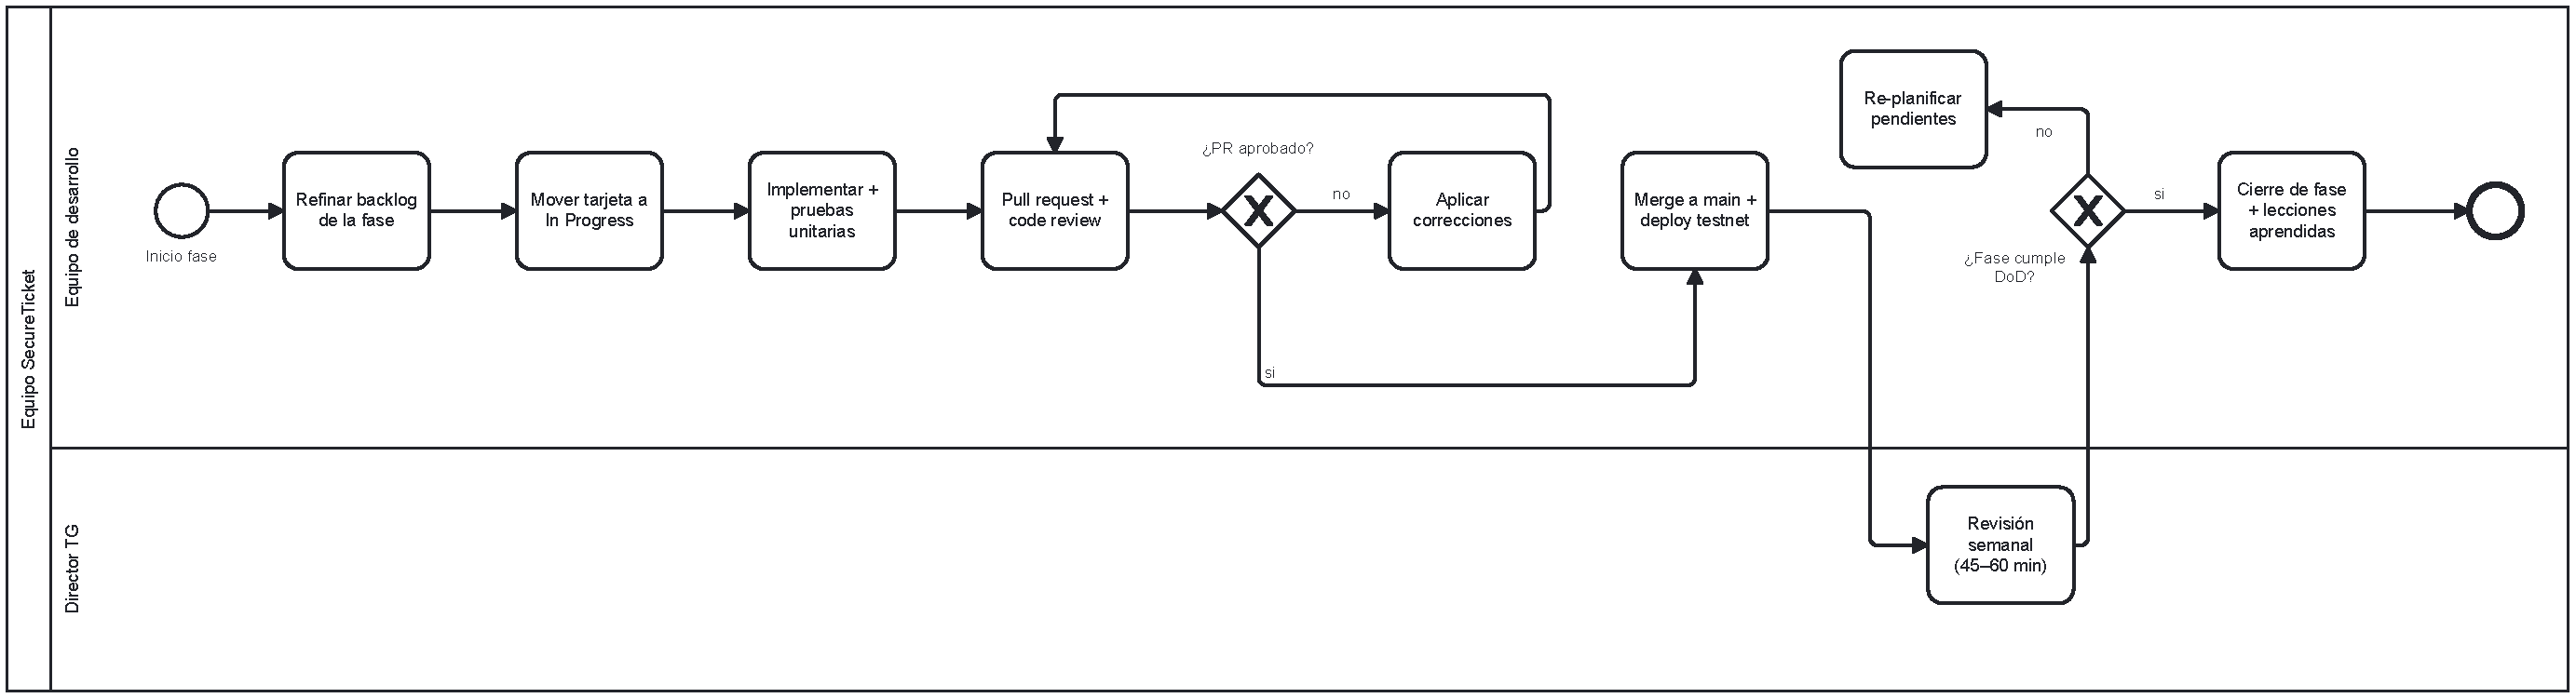
\includegraphics[width=0.95\linewidth]{diagrams/bpmn-ciclo-vida.pdf}
        \caption{Flujo BPMN del ciclo de vida — iteración Kanban con revisión semanal del director.}
        \label{fig:bpmn-ciclo-vida}
      \end{figure}

      La elección responde a tres factores específicos del proyecto:
      \begin{itemize}
        \item \textbf{Dedicación parcial} de los cuatro integrantes (proyecto académico paralelo a otras asignaturas), incompatible con \textit{sprints} de duración fija.
        \item \textbf{Alta incertidumbre técnica} en la integración con Soroban (SDK aún en evolución, comportamientos no documentados de la \textit{testnet}, ajuste de \textit{trustlines} y \textit{salt} en el despliegue), que exigía flujo continuo y respuesta rápida ante bloqueos.
        \item \textbf{Necesidad de iterar artefactos académicos} (SRS, SDD, SPMP) en paralelo con el código, sin congelar el alcance en fases rígidas.
      \end{itemize}

      \subsubsection{Fases del ciclo de vida ejecutadas}
      Aunque el trabajo diario se gestionó con flujo continuo, se identificaron \textbf{ocho fases incrementales} que estructuraron el proyecto en el semestre 2026-1 (ver Tabla~\ref{tab:fases-hitos}). Las fases se solaparon parcialmente: por ejemplo, el desarrollo del backend (semanas 7--11) comenzó antes de finalizar la implementación de contratos (semanas 6--9).

      \subsubsection{Prácticas Kanban aplicadas}
      \begin{itemize}
        \item \textbf{Tablero Kanban} en GitHub Projects, con columnas: \textit{Backlog} $\rightarrow$ \textit{To Do} $\rightarrow$ \textit{In Progress} $\rightarrow$ \textit{In Review} $\rightarrow$ \textit{Done}.
        \item \textbf{Límite WIP} de 2 tareas activas por integrante para evitar dispersión y favorecer cierres efectivos.
        \item \textbf{Definition of Done (DoD):} criterios mínimos para cerrar una tarea: código en \textit{main} mediante \textit{pull request}, pruebas pasando, revisión por al menos un compañero distinto al autor, y actualización de documentación cuando aplique.
        \item \textbf{Ceremonias ligeras:}
          \begin{itemize}
            \item \textit{Stand-up} asíncrono diario por canal de mensajería (3 preguntas: qué hice ayer, qué haré hoy, qué me bloquea).
            \item Revisión semanal con el director (Rafael V. Páez), de 45--60 min, donde se revisaban avances, riesgos y artefactos.
            \item Revisión interna del equipo al cierre de cada fase incremental, para consolidar lecciones aprendidas.
          \end{itemize}
        \item \textbf{Integración continua manual:} compilación y ejecución de pruebas antes de cada \textit{merge} a \textit{main}; despliegue manual a \textit{testnet} cuando aplicaba.
      \end{itemize}

      \subsubsection{Análisis de Alternativas y Justificación}
      \label{subsubsec:analisis-ciclo-vida}

      Antes de adoptar el enfoque \textbf{ágil con tablero Kanban}, el equipo evaluó cuatro modelos de ciclo de vida candidatos. La Tabla~\ref{tab:alt-ciclo-vida} resume el análisis comparativo frente a los \textit{drivers} del proyecto: equipo de cinco estudiantes con disponibilidad parcial, requisitos cambiantes derivados de un dominio (Web3) desconocido para el equipo, calendario fijo de 16~semanas con cierre el 24 de mayo de 2026 y necesidad de retroalimentación semanal con el director.

      \begin{longtable}{@{}p{3.0cm} p{4.5cm} p{4.0cm} p{3.0cm}@{}}
        \caption{Análisis de alternativas de modelo de ciclo de vida}
        \label{tab:alt-ciclo-vida}\\
        \toprule
        \textbf{Modelo} & \textbf{Fortalezas} & \textbf{Debilidades en este proyecto} & \textbf{Veredicto}\\
        \midrule
        \endfirsthead
        \toprule
        \textbf{Modelo} & \textbf{Fortalezas} & \textbf{Debilidades} & \textbf{Veredicto}\\
        \midrule
        \endhead
        \bottomrule
        \endfoot
        Cascada \cite{royce1970} & Trazabilidad fuerte; documentación completa por fase. & Asume requisitos estables; cualquier cambio en SRS obliga a re-trabajo masivo. No tolera el descubrimiento progresivo en Soroban. & Descartado\\
        RUP \cite{kruchten2003} & Iterativo; vistas arquitectónicas (4+1); hitos de control bien definidos. & Sobrecarga documental excesiva para un equipo de cinco; demasiados roles formales. & Descartado\\
        Scrum \cite{schwaber2020} & Ritmo iterativo; retrospectivas; \textit{product backlog} priorizado. & \textit{Sprints} de duración fija chocan con horarios académicos heterogéneos del equipo; \textit{Sprint Planning} y \textit{Review} de tamaño fijo no se acomodan a semanas con parciales o receso. & Parcialmente aplicable\\
        Kanban \cite{anderson2010,brechner2015} & Flujo continuo; WIP limitado; ceremonias ligeras; permite incorporar la revisión semanal con el director como cadencia natural. & Sin \textit{sprints} explícitos, exige mayor disciplina para evitar tareas estancadas. & \textbf{Seleccionado}\\
      \end{longtable}

      \paragraph{Justificación.} Kanban resultó la mejor alternativa por tres razones, soportadas en la literatura:
      \begin{enumerate}
        \item \textbf{Flujo continuo sin \textit{sprints} fijos:} Anderson \cite{anderson2010} y Brechner \cite{brechner2015} muestran que Kanban se acomoda mejor a equipos con disponibilidad heterogénea y a dominios con alta tasa de descubrimiento, como el desarrollo sobre Soroban (tecnología relativamente nueva, documentación en evolución \cite{stellardocs}).
        \item \textbf{WIP limitado como mecanismo de control:} limitar el trabajo en curso a dos tarjetas por integrante redujo el \textit{cycle time} promedio y evitó el bloqueo por tareas a medio terminar antes de parciales o semana santa.
        \item \textbf{Compatibilidad con el ciclo incremental:} sobre Kanban se mantuvo un ciclo \textbf{incremental} de cuatro fases (Fundamentos~$\rightarrow$~Reventa~$\rightarrow$~Verificación~$\rightarrow$~Panel admin), cada una validada en \textit{testnet} con el director. Esto preserva los hitos del calendario académico sin imponer la rigidez de los \textit{sprints} de Scrum.
      \end{enumerate}

      Las prácticas específicas del equipo (revisión por pares, \textit{trunk-based development}, \textit{test-driven mindset} en contratos, T-shirt sizing) se detallan en la Sección~\ref{subsec:herramientas} y son consistentes con las recomendaciones de \cite{anderson2010,beck2002,humble2010}.

    \subsection{Métodos, lenguajes y herramientas}
    \label{subsec:herramientas}

      \subsubsection{Lenguajes de programación}
      \begin{itemize}
        \item \textbf{Rust} (con \texttt{soroban-sdk 23}): contratos inteligentes en Soroban; compilación a WebAssembly con \texttt{cargo build --release --target wasm32v1-none}.
        \item \textbf{TypeScript} (Node 20): backend con Express + Prisma, indexer y \textit{scripts} de despliegue.
        \item \textbf{TypeScript / JavaScript} (React 18 + Vite): frontend SPA.
        \item \textbf{SQL} (PostgreSQL 15 en Supabase): consultas analíticas y migraciones gestionadas con Prisma.
      \end{itemize}

      \subsubsection{Herramientas técnicas}
      La Tabla~\ref{tab:herramientas-tecnicas} consolida las herramientas técnicas utilizadas, agrupadas por categoría.

      \begin{longtable}{@{}p{3.3cm} p{4.0cm} p{7.5cm}@{}}
        \caption{Herramientas técnicas del proyecto}
        \label{tab:herramientas-tecnicas}\\
        \toprule
        \textbf{Categoría} & \textbf{Herramienta} & \textbf{Uso en el proyecto}\\
        \midrule
        \endfirsthead
        \toprule
        \textbf{Categoría} & \textbf{Herramienta} & \textbf{Uso en el proyecto}\\
        \midrule
        \endhead
        \bottomrule
        \endfoot
        Contratos & Soroban SDK 23 (Rust) & Implementación de \texttt{event\_contract}, \texttt{factory\_contract} y \texttt{ticket\_nft\_contract}.\\
        Contratos & Stellar CLI / soroban-cli & Compilación, despliegue e invocación en \textit{testnet}.\\
        Backend & Node.js 20 + Express & API REST.\\
        Backend & Prisma ORM & Modelado de datos, migraciones y \textit{type-safety} contra PostgreSQL.\\
        Backend & Stellar SDK (JS) & Construcción de XDR, firma y envío de transacciones.\\
        Frontend & React 18 + Vite & SPA y \textit{tooling} de desarrollo.\\
        Frontend & Freighter Wallet & Firma de transacciones no-custodial por parte del usuario.\\
        Frontend & html5-qrcode & Escáner QR para verificación de boletos en puerta.\\
        Datos & PostgreSQL 15 (Supabase) & Base de datos transaccional \textit{off-chain}.\\
        Blockchain & Stellar \textit{testnet} & Red de pruebas para contratos y transacciones.\\
        Blockchain & Soroban RPC + Horizon & Endpoints consumidos por backend e indexer.\\
        Despliegue & Vercel & Hosting del frontend.\\
        Despliegue & Railway / Render & Hosting del backend y del indexer.\\
        VCS & Git + GitHub & Control de versiones, \textit{pull requests} y revisiones de código.\\
        Gestión & GitHub Projects (Kanban) & Tablero de tareas, asignación y seguimiento WIP.\\
        Comunicación & WhatsApp + Discord & Mensajería diaria y canales temáticos por subsistema.\\
        Reuniones & Microsoft Teams / Google Meet & Revisiones semanales con el director y reuniones internas.\\
        Documentación & \LaTeX{} (MiKTeX, TeXstudio) & Memoria de TG, Plan de Proyecto, SRS, SDD, Propuesta y Formato de Biblioteca.\\
        Diagramas & draw.io / PlantUML & Diagramas C4, BPMN y de secuencia.\\
      \end{longtable}

      \subsubsection{Métodos y técnicas}
      \begin{itemize}
        \item \textbf{Modelo C4} (Simon Brown) para representar la arquitectura en niveles de contexto, contenedores y despliegue (ver SDD).
        \item \textbf{Test-driven mindset} en contratos: cada función pública de \texttt{event\_contract} cuenta con al menos un caso de prueba unitario que cubre la ruta positiva y los errores tipados.
        \item \textbf{Trunk-based development} con \textit{feature branches} de corta duración y \textit{pull requests} hacia \texttt{main}.
        \item \textbf{Revisión por pares} obligatoria antes de \textit{merge}.
        \item \textbf{Estimación relativa} con \textit{T-shirt sizing} (S/M/L/XL) en lugar de \textit{story points} numéricos, dada la naturaleza académica del proyecto.
      \end{itemize}

      \subsubsection{Análisis de Alternativas y Justificación}
      \label{subsubsec:analisis-herramientas}

      Las decisiones tecnológicas más críticas (plataforma de \textit{smart contracts}, \textit{framework} frontend, base de datos, modelo de billetera) se tomaron tras evaluar alternativas frente a tres criterios: \emph{compatibilidad con Web2.5}, \emph{costo operativo en testnet/mainnet} y \emph{curva de aprendizaje aceptable para un equipo académico de cinco}. La Tabla~\ref{tab:alt-herramientas} resume el análisis.

      \begin{longtable}{@{}p{2.8cm} p{3.4cm} p{4.2cm} p{4.0cm}@{}}
        \caption{Análisis de alternativas tecnológicas principales}
        \label{tab:alt-herramientas}\\
        \toprule
        \textbf{Decisión} & \textbf{Alternativas} & \textbf{Argumentos descartados} & \textbf{Elegido}\\
        \midrule
        \endfirsthead
        \toprule
        \textbf{Decisión} & \textbf{Alternativas} & \textbf{Argumentos descartados} & \textbf{Elegido}\\
        \midrule
        \endhead
        \bottomrule
        \endfoot
        Plataforma de \textit{smart contracts} & Ethereum/Solidity \cite{wood2014,solidity}, Solana/Anchor \cite{solanadocs}, Stellar/Soroban \cite{stellardocs,sorobandocs} & Ethereum: \textit{gas fees} altas en \textit{mainnet} y experiencia de usuario costosa para boletería de bajo ticket. Solana: ecosistema Rust maduro pero finalidad y herramientas de billetera menos amigables para Web2.5. & \textbf{Stellar/Soroban}: \textit{fees} bajas, finalidad de 5\,s, billetera Freighter no-custodial, estándar SEP-41 para activos.\\
        Lenguaje de contratos & Solidity (EVM) \cite{solidity}, Move \cite{movebook}, Rust+Soroban \cite{klabnik2023} & Solidity: trampas conocidas de \textit{reentrancy} y manejo manual de \textit{overflow}. Move: ecosistema pequeño y sin soporte en Stellar. & \textbf{Rust} con \texttt{soroban-sdk}: tipado fuerte, \texttt{cargo test} integrado, errores tipados.\\
        Frontend & Vue~3 \cite{vuedocs}, Svelte \cite{sveltedocs}, React+Vite \cite{reactdocs,vitedocs} & Vue: experiencia previa del equipo nula. Svelte: comunidad menor y menos integraciones con Stellar SDK. & \textbf{React+Vite}: ecosistema maduro, Stellar SDK JS bien documentado, Vercel deploy nativo.\\
        Backend & Spring Boot \cite{springdocs}, Django \cite{djangodocs}, Express+Prisma \cite{expressdocs,prismadocs} & Spring/Django: pesados para un proxy XDR \textit{stateless}; añaden tiempos de \textit{build}. & \textbf{Node/Express+Prisma}: comparte TypeScript con el frontend; Prisma da migraciones tipadas.\\
        Base de datos & MongoDB \cite{mongodocs}, MySQL, PostgreSQL/Supabase \cite{postgresdocs,supabasedocs} & MongoDB: relaciones evento-boleto-usuario son fuertemente relacionales. MySQL: sin plan gratuito con \textit{backups} automáticos cómodo. & \textbf{PostgreSQL gestionado por Supabase}: \textit{backups} diarios, autenticación integrada.\\
        Modelo de billetera & Custodia centralizada, MetaMask Snaps, Freighter \cite{freighter} & Custodia: obligaría a manejar llaves privadas en el backend (riesgo legal/seguridad). MetaMask Snap: sin soporte estable para Soroban a la fecha del proyecto. & \textbf{Freighter Wallet}: no-custodial, firma local del usuario, integración oficial Stellar.\\
        \textit{Hosting} & AWS \cite{awsdocs}, Render, Vercel+Railway \cite{verceldocs,railwaydocs} & AWS: complejidad operativa y costos imprevisibles para un proyecto académico. & \textbf{Vercel} (frontend) + \textbf{Railway} (backend+indexer): planes gratuitos suficientes y CI/CD integrado con GitHub.\\
      \end{longtable}

      \paragraph{Justificación global.} La combinación \textbf{Stellar/Soroban + Rust + Freighter + React + Express/Prisma + Supabase + Vercel/Railway} satisface los tres criterios: (i)~Web2.5 viable porque la billetera es opcional y el indexer mantiene una vista off-chain consultable sin firma; (ii)~costo operativo nulo dentro de los planes gratuitos durante el semestre (los servicios públicos del equipo son el único gasto real); y (iii)~curva de aprendizaje manejable porque cuatro de los siete componentes (React, Express, Prisma, PostgreSQL) ya formaban parte del bagaje previo del equipo, concentrando el esfuerzo de aprendizaje en Rust/Soroban (un único \textit{driver} dominante, mitigado con los recursos formativos oficiales \cite{sorobandocs,klabnik2023}).

    \subsection{Plan de aceptación del producto}
    \label{subsec:plan-aceptacion}

      El producto entregado se valida formalmente contra los \textbf{criterios de aceptación} definidos en el SRS y refinados en cada revisión semanal con el director. El plan de aceptación distingue tres niveles de validación.

      \subsubsection{Niveles de validación}
      \begin{enumerate}
        \item \textbf{Validación técnica (interna del equipo):} ejecución exitosa de las suites de pruebas (unitarias en Rust, integración en Node y E2E desde el frontend) sobre la rama \texttt{main}, sin defectos críticos abiertos al cierre de la fase.
        \item \textbf{Validación funcional (revisión con el director):} demostración semanal del estado del flujo E2E sobre la \textit{testnet} (compra, asegurar en blockchain, reventa P2P, verificación en puerta), validando que los criterios de aceptación del SRS se cumplen tal como están escritos.
        \item \textbf{Aceptación final (entrega y sustentación):} entrega del paquete final de seis documentos (Memoria, Plan de Proyecto, SRS, SDD, Propuesta y Formato de Biblioteca) a la coordinación académica el \textbf{24 de mayo de 2026}, y posterior sustentación ante el director y los jurados del trabajo de grado en una fecha asignada por la coordinación dentro de la ventana \textbf{25 de mayo -- 5 de junio de 2026}, con el sistema desplegado en \textit{testnet}.
      \end{enumerate}

      \subsubsection{Criterios de aceptación globales}
      Para considerar el producto aceptado se requirió el cumplimiento de los siguientes criterios:
      \begin{itemize}
        \item \textbf{Suite de contratos desplegada:} \texttt{event\_contract}, \texttt{factory\_contract} y \texttt{ticket\_nft\_contract} desplegados en \textit{testnet} con direcciones verificables y al menos un evento operativo.
        \item \textbf{Flujo E2E completo:} un usuario autenticado puede navegar el catálogo, comprar un boleto (Web2), asegurarlo on-chain (Web3), revenderlo a otro usuario (\textit{burn}/\textit{remint} con comisiones) y un verificador autorizado puede redimirlo en puerta (escáner QR).
        \item \textbf{Cobertura de pruebas mínima:} todas las funciones públicas de los contratos tienen al menos un caso de prueba; el backend cubre las rutas críticas con pruebas de integración.
        \item \textbf{Documentación completa:} los seis documentos académicos entregables se encuentran finalizados, revisados y consistentes entre sí.
        \item \textbf{Sin defectos críticos abiertos:} cualquier defecto que impida la ejecución del flujo E2E está corregido al cierre del proyecto.
      \end{itemize}

      \subsubsection{Procedimiento de aceptación}
      \begin{enumerate}
        \item Al cierre de cada fase incremental, el equipo ejecuta la suite de pruebas y registra evidencias.
        \item En la revisión semanal con el director, se demuestra el avance sobre la \textit{testnet}; el director acepta o solicita correcciones.
        \item El paquete final de documentos se envía con al menos una semana de antelación a la sustentación, para revisión previa del director.
        \item En la sustentación, los jurados validan funcionalidad y documentación; el equipo atiende observaciones y aplica correcciones menores si aplica.
      \end{enumerate}

    \subsection{Estructura organizacional}
    \label{subsec:organizacion}

      \subsubsection{Interfaces externas}
      El proyecto se relaciona con los siguientes actores externos al equipo:
      \begin{itemize}
        \item \textbf{Director de trabajo de grado:} Rafael Vicente Páez Méndez, PhD. Aprueba alcance, valida avances semanalmente y firma los entregables académicos.
        \item \textbf{Jurados del trabajo de grado:} docentes asignados por la Universidad para la sustentación final.
        \item \textbf{Coordinación académica} de Ingeniería de Sistemas, Pontificia Universidad Javeriana Bogotá: define el calendario académico oficial y los formatos institucionales.
        \item \textbf{Comunidad Stellar / Soroban:} fuente de documentación técnica, foros de soporte y actualizaciones del SDK.
      \end{itemize}

      \subsubsection{Estructura interna del equipo}
      El equipo (Grupo 12) se organiza como una célula \textbf{auto-gestionada de cuatro integrantes} bajo coordinación de un PM, sin jerarquías formales. Las decisiones técnicas y de alcance se toman por consenso en las reuniones semanales internas; el PM resuelve empates cuando es necesario y representa al equipo ante el director.

      La Tabla~\ref{tab:roles-responsabilidades} resume los roles y responsabilidades principales por integrante.

      \begin{longtable}{@{}p{4.0cm} p{3.6cm} p{7.2cm}@{}}
        \caption{Roles y responsabilidades del equipo}
        \label{tab:roles-responsabilidades}\\
        \toprule
        \textbf{Integrante} & \textbf{Rol principal} & \textbf{Responsabilidades}\\
        \midrule
        \endfirsthead
        \toprule
        \textbf{Integrante} & \textbf{Rol principal} & \textbf{Responsabilidades}\\
        \midrule
        \endhead
        \bottomrule
        \endfoot
        Andrés Felipe Manosalva Garzón & PM / Coordinación & Coordinación del equipo, planificación, seguimiento del tablero Kanban, comunicación con el director, mantenimiento del SPMP y apoyo transversal en frontend y documentación.\\
        Santiago Andrés Mesa Niño & Blockchain (Soroban) & Diseño e implementación de los contratos en Rust, pruebas unitarias, despliegue en \textit{testnet} y mantenimiento de los \textit{scripts} de \textit{deploy}.\\
        Juan Diego Arias Durán & Backend & Diseño e implementación de la API Express + Prisma, XDR proxy, indexer Soroban, esquema PostgreSQL y arreglos puntuales en el frontend.\\
        Juan Camilo Carvajal Rodríguez & Frontend + QA/DevOps & Implementación de la SPA React/Vite, integración Freighter, escáner QR, ejecución de pruebas E2E y despliegues a Vercel/Railway.\\
      \end{longtable}

      \subsubsection{Matriz de responsabilidades (RACI resumida)}
      Una \textbf{matriz RACI} es una herramienta clásica de gestión de proyectos que clarifica, para cada entregable, el grado de involucramiento de cada persona u rol. Las siglas \textbf{R}, \textbf{A}, \textbf{C}, \textbf{I} corresponden a cuatro tipos distintos de responsabilidad, descritos a continuación:

      \begin{itemize}
        \item \textbf{R --- Responsible (Responsable de ejecutar).} Persona(s) que \textbf{realiza(n) el trabajo}. Es quien ``mete las manos'' en la tarea. Puede haber más de un \textbf{R} por entregable cuando el trabajo es compartido.
        \item \textbf{A --- Accountable (Aprobador / Rinde cuentas).} Persona que \textbf{aprueba el resultado final} y responde por él ante terceros. Debe existir \textbf{exactamente un A} por entregable para evitar diluir la responsabilidad. En este proyecto, el director del trabajo de grado es siempre el \textbf{A} de los entregables académicos.
        \item \textbf{C --- Consulted (Consultado).} Persona(s) cuya \textbf{opinión técnica se consulta antes de tomar decisiones} sobre el entregable. La consulta es \textit{bidireccional}: hay diálogo. Suelen ser expertos en el subsistema afectado.
        \item \textbf{I --- Informed (Informado).} Persona(s) a las que se les \textbf{comunica el resultado} una vez tomada la decisión o avanzado el trabajo, pero sin consulta previa. La comunicación es \textit{unidireccional}.
      \end{itemize}

      \textbf{Cómo leer la matriz:} cada fila representa un entregable y cada columna una persona. La celda indica qué tipo de involucramiento tiene esa persona con ese entregable. Por ejemplo, en la fila ``Contratos Soroban'': \textbf{SM} es \textbf{R} (Santiago ejecuta el trabajo), \textbf{AM} y \textbf{JA} son \textbf{C} (se consulta a Andrés por temas de planeación y a Juan Diego por la integración con el backend), \textbf{JC} es \textbf{I} (se le informa del avance) y el \textbf{Dir.} es \textbf{A} (el director aprueba el resultado final).

      Para abreviar se usan iniciales: \textbf{AM} (Andrés Manosalva), \textbf{SM} (Santiago Mesa), \textbf{JA} (Juan Diego Arias), \textbf{JC} (Juan Camilo Carvajal) y \textbf{Dir.} (Director del trabajo de grado).

      \begin{longtable}{@{}p{4.8cm} c c c c c@{}}
        \caption{Matriz RACI por entregable principal}
        \label{tab:raci}\\
        \toprule
        \textbf{Entregable} & \textbf{AM} & \textbf{SM} & \textbf{JA} & \textbf{JC} & \textbf{Dir.}\\
        \midrule
        \endfirsthead
        \toprule
        \textbf{Entregable} & \textbf{AM} & \textbf{SM} & \textbf{JA} & \textbf{JC} & \textbf{Dir.}\\
        \midrule
        \endhead
        \bottomrule
        \endfoot
        Contratos Soroban & C & R & C & I & A\\
        Backend + Indexer & C & C & R & I & A\\
        Frontend + Freighter & C & I & C & R & A\\
        Despliegue \textit{testnet} (12 eventos) & C & C & C & R & A\\
        Plan de Proyecto (SPMP) & R & I & C & I & A\\
        SRS & R & C & C & C & A\\
        SDD & C & C & R & C & A\\
        Memoria de TG & R & C & C & C & A\\
        Propuesta de TG & R & I & I & I & A\\
        Formato de Biblioteca & R & I & I & I & A\\
        Demo final & C & C & C & R & A\\
      \end{longtable}

      \subsubsection{Canales de comunicación}
      \begin{itemize}
        \item \textbf{Mensajería diaria:} grupo de WhatsApp del equipo para coordinación rápida y \textit{stand-up} asíncrono.
        \item \textbf{Discord:} canales temáticos por subsistema (\textit{contracts}, \textit{backend}, \textit{frontend}, \textit{docs}) para discusiones técnicas más extensas.
        \item \textbf{GitHub Issues / Pull Requests:} discusión formal asociada al código, decisiones de diseño y revisiones.
        \item \textbf{Microsoft Teams / Google Meet:} reuniones semanales con el director y reuniones de cierre de fase del equipo.
        \item \textbf{Correo institucional:} comunicación formal con coordinación académica y entrega de documentos a la Universidad.
      \end{itemize}

  % =========================================================
  % SECCIÓN 9 — Administración del proyecto
  % =========================================================
  \section{Administración del proyecto}
  \label{sec:administracion}

    Esta sección documenta cómo se administró el proyecto durante el semestre 2026-1: los métodos y herramientas de estimación de esfuerzo, el plan de inicio (entrenamiento e infraestructura) y los planes de trabajo detallados (estructura desglosada del trabajo, carta Gantt, asignación de recursos y presupuesto consolidado).

    \subsection{Métodos y herramientas de estimación}
    \label{subsec:estimacion}

      \subsubsection{Enfoque general}
      Dada la naturaleza académica del proyecto y la dedicación parcial del equipo, no se aplicaron técnicas formales de estimación paramétrica (COCOMO, Function Points). En su lugar, se combinaron dos técnicas ágiles ampliamente aceptadas para equipos pequeños:
      \begin{itemize}
        \item \textbf{T-shirt sizing} (S/M/L/XL) para clasificar tareas del \textit{backlog} según el esfuerzo relativo percibido por el integrante con mayor experiencia técnica en el área correspondiente.
        \item \textbf{Estimación por analogía:} comparación con tareas similares ya completadas dentro del proyecto (por ejemplo, estimar el tiempo de una nueva función del contrato a partir de las funciones implementadas y probadas con anterioridad).
      \end{itemize}

      La correspondencia aproximada entre tallas y horas-persona se muestra en la Tabla~\ref{tab:tshirt-sizing}. Esta correspondencia se calibró durante las primeras dos fases del proyecto y se mantuvo estable hasta el cierre.

      \begin{table}[H]
        \centering
        \begin{tabular}{@{}c r p{8.0cm}@{}}
          \toprule
          \textbf{Talla} & \textbf{Horas} & \textbf{Ejemplo típico}\\
          \midrule
          S  & 1--2  & Ajuste de estilos en una pantalla del frontend; corrección de un texto del SRS.\\
          M  & 3--5  & Implementación de un \textit{endpoint} REST con pruebas básicas; un caso de prueba de contrato.\\
          L  & 6--10 & Una función pública nueva del \texttt{event\_contract} con su batería de pruebas.\\
          XL & 11+   & Indexer Soroban; \textit{burn}/\textit{remint} atómico; integración completa de Freighter.\\
          \bottomrule
        \end{tabular}
        \caption{Correspondencia T-shirt sizing $\leftrightarrow$ horas-persona}
        \label{tab:tshirt-sizing}
      \end{table}

      \subsubsection{Herramientas de estimación y seguimiento}
      \begin{itemize}
        \item \textbf{GitHub Projects} (Kanban): cada tarjeta del tablero registra su talla estimada como etiqueta (\texttt{size: S/M/L/XL}).
        \item \textbf{Hoja de cálculo de horas} compartida en Google Drive: cada integrante registra semanalmente las horas reales invertidas por tarea, permitiendo calibrar la estimación.
        \item \textbf{Issues de GitHub}: las tareas complejas se descomponen en \textit{checklists} antes de empezar, lo que reduce el sesgo optimista en la estimación.
      \end{itemize}

      \subsubsection{Calibración y aprendizajes}
      Las primeras tres iteraciones del proyecto presentaron una desviación promedio de $+30\%$ entre las horas estimadas y las horas reales, especialmente en tareas relacionadas con Soroban (debido a la curva de aprendizaje del SDK y problemas no documentados con el \textit{target} \texttt{wasm32v1-none}). A partir de la fase de implementación del backend, la desviación bajó a $\sim$$10\%$ gracias a la calibración de las tallas y a la práctica acumulada del equipo.

    \subsection{Plan de inicio del proyecto}
    \label{subsec:plan-inicio}

      El plan de inicio define las actividades ejecutadas durante las dos primeras semanas (\textbf{semanas 1--2 del semestre 2026-1}) para habilitar al equipo y la infraestructura antes de empezar el desarrollo.

      \subsubsection{Entrenamiento y nivelación}
      Las áreas técnicas con mayor incertidumbre exigieron una fase explícita de capacitación:
      \begin{itemize}
        \item \textbf{Stellar y Soroban:} lectura de la documentación oficial (\textit{Stellar Documentation}, \textit{Soroban Smart Contract Reference}), realización del \textit{tutorial} oficial \textit{``Hello World''} de Soroban y revisión de los \textit{contracts examples} del repositorio público de Stellar. Responsable: Santiago Mesa (Blockchain); apoyo de todo el equipo.
        \item \textbf{Freighter Wallet:} estudio del SDK \textit{Freighter API} y pruebas locales de firma de transacciones. Responsable: Juan Camilo Carvajal (Frontend).
        \item \textbf{Prisma + Supabase:} revisión de la documentación de Prisma 5, ejecución de migraciones de ejemplo contra una instancia gratuita de Supabase. Responsable: Juan Diego Arias (Backend).
        \item \textbf{Patrones y metodologías:} repaso interno del modelo C4, del estándar IEEE 1058 (este documento) y del flujo Kanban. Responsable: Andrés Manosalva (PM); difusión a todo el equipo.
      \end{itemize}

      \subsubsection{Infraestructura inicial}
      Durante las semanas 1--2 también se aprovisionó la infraestructura mínima necesaria para arrancar:
      \begin{itemize}
        \item \textbf{Repositorio Git} en GitHub bajo la organización \textit{Tesis-Stellar} con el nombre \textit{Secure-Ticket}; configuración de ramas protegidas (\texttt{main}), plantillas de \textit{pull request} y archivo \texttt{CODEOWNERS}.
        \item \textbf{Tablero Kanban} en GitHub Projects con columnas \textit{Backlog $\rightarrow$ To Do $\rightarrow$ In Progress $\rightarrow$ In Review $\rightarrow$ Done} y etiquetas por subsistema (\texttt{contracts}, \texttt{backend}, \texttt{frontend}, \texttt{docs}, \texttt{infra}).
        \item \textbf{Cuentas y proyectos} creados en: Supabase (PostgreSQL), Vercel (frontend), Railway (backend e indexer); todos en planes \textit{free tier} académicos.
        \item \textbf{Wallets de testnet} generadas para los roles del sistema: \texttt{ADMIN}, \texttt{ORGANIZER}, \texttt{PLATFORM}, \texttt{BUYER1}, \texttt{BUYER2}, \texttt{VERIFIER}; semillas de 12 palabras almacenadas en \texttt{backend/.env.deploy} (\textit{gitignored}).
        \item \textbf{Entorno local} unificado: documento \texttt{SETUP.md} con instrucciones para Rust + cargo, Node 20, soroban-cli y configuración de Freighter en modo \textit{testnet}.
        \item \textbf{Carpeta compartida en Google Drive} para los borradores LaTeX y materiales de apoyo.
      \end{itemize}

    \subsection{Planes de trabajo}
    \label{subsec:planes-trabajo}

      \subsubsection{Estructura desglosada del trabajo (WBS)}
      \label{subsubsec:wbs}
      La WBS organiza el trabajo del proyecto en tres niveles jerárquicos: \textbf{nivel 1} (proyecto), \textbf{nivel 2} (paquetes de trabajo por subsistema o tipo de artefacto) y \textbf{nivel 3} (entregables o componentes específicos). El esquema se presenta a continuación.

      \begin{enumerate}[label=\textbf{1.\arabic*},leftmargin=*]
        \item \textbf{Gestión del proyecto}
          \begin{itemize}[label=$\circ$]
            \item Plan de Proyecto (SPMP) y sus versiones (v1.0 a v1.5).
            \item Tablero Kanban y seguimiento semanal.
            \item Revisiones semanales con el director y actas internas.
            \item Cierre del proyecto y \textit{post-mortem}.
          \end{itemize}
        \item \textbf{Análisis y diseño}
          \begin{itemize}[label=$\circ$]
            \item Requisitos funcionales y no funcionales (SRS).
            \item Modelo de dominio Web2.5 (catálogo, carrito, boleto, NFT, evento, comisiones).
            \item Vistas C4 (contexto, contenedores, despliegue) y diagramas de secuencia.
            \item Modelo de datos on-chain (\textit{storage keys}, eventos) y off-chain (Prisma schema).
            \item SDD (Especificación del Diseño).
          \end{itemize}
        \item \textbf{Contratos inteligentes (Soroban / Rust)}
          \begin{itemize}[label=$\circ$]
            \item \texttt{event\_contract}: emisión, listado, compra primaria, reventa \textit{burn}/\textit{remint}, verificadores, redención, invalidación.
            \item \texttt{factory\_contract}: patrón Factory por evento.
            \item \texttt{ticket\_nft\_contract}: NFT SEP-41 para Freighter Collectibles.
            \item Pruebas unitarias e integración (Rust \texttt{\#[test]}).
            \item Scripts de despliegue y configuración de \texttt{testnet}.
          \end{itemize}
        \item \textbf{Backend (Express + Prisma + Indexer)}
          \begin{itemize}[label=$\circ$]
            \item API REST: catálogo, autenticación (bcrypt+JWT), carrito, \textit{checkout}, órdenes, boletos.
            \item Constructor de XDR \textit{stateless} (XDR proxy).
            \item Indexer Soroban (polling cada 5 s) y sincronización a PostgreSQL.
            \item Esquema Prisma y migraciones versionadas.
            \item Documentación de endpoints.
          \end{itemize}
        \item \textbf{Frontend (React + Vite)}
          \begin{itemize}[label=$\circ$]
            \item Catálogo, detalle de evento, carrito y \textit{checkout}.
            \item Cuenta de usuario, órdenes, boletos.
            \item Integración Freighter Wallet (conexión, firma, asegurar on-chain).
            \item Mercado secundario P2P (publicar reventa, comprar reventa, cancelar).
            \item Escáner QR para verificación en puerta.
            \item Panel de administración (Phase 4) y vistas para rol STAFF.
          \end{itemize}
        \item \textbf{Pruebas y aseguramiento de calidad}
          \begin{itemize}[label=$\circ$]
            \item Plan y casos de prueba.
            \item Ejecución de pruebas unitarias, integración y E2E.
            \item Evidencias y reporte de defectos.
            \item Validación contra los criterios de aceptación del SRS.
          \end{itemize}
        \item \textbf{Despliegue e infraestructura}
          \begin{itemize}[label=$\circ$]
            \item Despliegue de los 12 eventos demostrativos en \textit{testnet}.
            \item Configuración de Vercel (frontend), Railway (backend, indexer) y Supabase (PostgreSQL).
            \item Variables de entorno y secretos.
          \end{itemize}
        \item \textbf{Documentación académica final}
          \begin{itemize}[label=$\circ$]
            \item Memoria de TG.
            \item Propuesta de TG.
            \item SRS final.
            \item SDD final.
            \item Plan de Proyecto v1.5 (este documento).
            \item Formato de Biblioteca.
          \end{itemize}
        \item \textbf{Demo y sustentación final}
          \begin{itemize}[label=$\circ$]
            \item Guion del demo (flujo E2E sobre \textit{testnet}).
            \item Grabación opcional en video del recorrido.
            \item Sustentación ante director y jurados (ventana 25 de mayo -- 5 de junio de 2026, fecha exacta por confirmar).
          \end{itemize}
      \end{enumerate}

      \subsubsection{Carta Gantt ejecutada}
      \label{subsubsec:gantt}
      La Tabla~\ref{tab:gantt} representa la carta Gantt del proyecto a nivel de paquete WBS y semana del semestre. Las celdas marcadas con un punto (\textbullet) indican semanas de actividad principal del paquete; el cierre y la entrega documental son el viernes \textbf{24 de mayo de 2026} (semana 16). La sustentación se programa en una fecha asignada por la coordinación dentro de la ventana \textbf{25 de mayo -- 5 de junio de 2026} y, por estar fuera del semestre académico, no se grafica en la carta Gantt.

      \begin{longtable}{@{}p{4.5cm}*{16}{c}@{}}
        \caption{Carta Gantt ejecutada (semanas 1--16 del semestre 2026-1)}
        \label{tab:gantt}\\
        \toprule
        \textbf{Paquete WBS} & \multicolumn{16}{c}{\textbf{Semana}}\\
        & 1 & 2 & 3 & 4 & 5 & 6 & 7 & 8 & 9 & 10 & 11 & 12 & 13 & 14 & 15 & 16\\
        \midrule
        \endfirsthead
        \toprule
        \textbf{Paquete WBS} & \multicolumn{16}{c}{\textbf{Semana}}\\
        & 1 & 2 & 3 & 4 & 5 & 6 & 7 & 8 & 9 & 10 & 11 & 12 & 13 & 14 & 15 & 16\\
        \midrule
        \endhead
        \bottomrule
        \endfoot
        1. Gestión          & \textbullet & \textbullet & \textbullet & \textbullet & \textbullet & \textbullet & \textbullet & \textbullet & \textbullet & \textbullet & \textbullet & \textbullet & \textbullet & \textbullet & \textbullet & \textbullet\\
        2. Análisis y diseño & \textbullet & \textbullet & \textbullet & \textbullet & \textbullet &   &   &   &   &   &   &   &   &   &   &  \\
        3. Contratos        &   &   &   &   &   & \textbullet & \textbullet & \textbullet & \textbullet &   &   &   &   &   &   &  \\
        4. Backend + Indexer &   &   &   &   &   &   & \textbullet & \textbullet & \textbullet & \textbullet & \textbullet &   &   &   &   &  \\
        5. Frontend         &   &   &   &   &   &   &   &   & \textbullet & \textbullet & \textbullet & \textbullet &   &   &   &  \\
        6. Pruebas/QA       &   &   &   &   &   &   &   &   &   &   &   &   &   & \textbullet & \textbullet &   \\
        7. Despliegue       &   &   &   &   &   &   &   &   &   &   &   & \textbullet & \textbullet & \textbullet & \textbullet &   \\
        8. Documentación final &   &   &   &   &   &   &   &   &   &   &   &   &   &   & \textbullet & \textbullet\\
        9. Demo / sustentación &   &   &   &   &   &   &   &   &   &   &   &   &   &   &   & \textbullet\\
      \end{longtable}

      \subsubsection{Asignación de recursos}
      \label{subsubsec:recursos}
      La asignación de recursos humanos al esfuerzo de cada paquete WBS se resume en la Tabla~\ref{tab:asignacion-recursos}. La columna \textit{Líder} indica el integrante responsable del paquete; las demás columnas indican el porcentaje aproximado del esfuerzo total del integrante dedicado a ese paquete.

      \begin{longtable}{@{}p{4.2cm} p{3.4cm} c c c c@{}}
        \caption{Asignación de recursos por paquete WBS (\% del esfuerzo del integrante)}
        \label{tab:asignacion-recursos}\\
        \toprule
        \textbf{Paquete WBS} & \textbf{Líder} & \textbf{AM} & \textbf{SM} & \textbf{JA} & \textbf{JC}\\
        \midrule
        \endfirsthead
        \toprule
        \textbf{Paquete WBS} & \textbf{Líder} & \textbf{AM} & \textbf{SM} & \textbf{JA} & \textbf{JC}\\
        \midrule
        \endhead
        \bottomrule
        \endfoot
        1. Gestión & AM & 35\% & 5\% & 5\% & 5\%\\
        2. Análisis y diseño & AM / JA & 20\% & 10\% & 20\% & 10\%\\
        3. Contratos Soroban & SM & 5\% & 55\% & 10\% & 5\%\\
        4. Backend + Indexer & JA & 5\% & 10\% & 40\% & 10\%\\
        5. Frontend & JC & 5\% & 5\% & 10\% & 35\%\\
        6. Pruebas y QA & JC & 10\% & 10\% & 5\% & 20\%\\
        7. Despliegue & JC & 5\% & 5\% & 5\% & 10\%\\
        8. Documentación final & AM & 10\% & --- & 5\% & 5\%\\
        9. Demo / sustentación & JC & 5\% & --- & --- & --- \\
        \midrule
        \textbf{Total} & & \textbf{100\%} & \textbf{100\%} & \textbf{100\%} & \textbf{100\%}\\
      \end{longtable}

      Convertido a horas-persona (a partir de la Tabla~\ref{tab:horas-persona}: AM 60~h, SM 65~h, JA 65~h, JC 65~h), el esfuerzo total invertido por paquete se muestra en la Tabla~\ref{tab:horas-paquete}.

      \begin{table}[H]
        \centering
        \begin{tabular}{@{}l r@{}}
          \toprule
          \textbf{Paquete WBS} & \textbf{Horas totales}\\
          \midrule
          1. Gestión & 30\\
          2. Análisis y diseño & 32\\
          3. Contratos Soroban & 45\\
          4. Backend + Indexer & 38\\
          5. Frontend & 32\\
          6. Pruebas y QA & 28\\
          7. Despliegue & 16\\
          8. Documentación final & 16\\
          9. Demo / sustentación & 3\\
          \midrule
          \textbf{Indirecto / reuniones / otros} & 15\\
          \midrule
          \textbf{Total} & \textbf{255}\\
          \bottomrule
        \end{tabular}
        \caption{Horas-persona ejecutadas por paquete WBS}
        \label{tab:horas-paquete}
      \end{table}

      \subsubsection{Presupuesto detallado}
      \label{subsubsec:presupuesto-detallado}
      El presupuesto monetario consolidado del proyecto se presentó en la Tabla~\ref{tab:costos-operativos} de la Sección~\ref{subsec:resumen-calendario-presupuesto} (total \textbf{748.000 COP}, con contingencia del 10\%). La Tabla~\ref{tab:presupuesto-fases} desagrega el gasto por fase del proyecto, vinculando los rubros operativos con el momento en que se incurrieron.

      \begin{table}[H]
        \centering
        \begin{tabular}{@{}p{5.0cm} p{5.5cm} r@{}}
          \toprule
          \textbf{Fase / Momento} & \textbf{Rubro} & \textbf{Monto (COP)}\\
          \midrule
          Semanas 1--16 (semestre) & Servicios de luz (4 hogares) & 480{,}000\\
          Semanas 3--13 (revisiones)& Transporte / viáticos & 60{,}000\\
          Semanas 15--16 (cierre) & Transporte / viáticos (sustentación) & 20{,}000\\
          Semana 16 (entrega) & Impresiones de anexos & 120{,}000\\
          \midrule
          \textbf{Subtotal operativo} & & \textbf{680{,}000}\\
          Reserva (contingencia 10\%) & Imprevistos & 68{,}000\\
          \midrule
          \textbf{Total} & & \textbf{748{,}000}\\
          \bottomrule
        \end{tabular}
        \caption{Presupuesto monetario desagregado por fase y rubro}
        \label{tab:presupuesto-fases}
      \end{table}

      \textbf{Observaciones de presupuesto:}
      \begin{itemize}
        \item El presupuesto se ejecutó \textbf{íntegramente dentro de lo planificado}, sin necesidad de activar la contingencia.
        \item Los servicios de luz se asumen como costo indirecto del trabajo desde casa, prorrateado por integrante.
        \item Los costos de hosting (Vercel, Railway, Supabase) y de licencias de herramientas (GitHub, Freighter, Stellar testnet) fueron \textbf{0 COP}, gracias a planes gratuitos.
        \item El equipo financió íntegramente los gastos operativos como aporte propio al trabajo de grado.
      \end{itemize}

  % =========================================================
  % SECCIÓN 10 — Monitoreo y control del proyecto
  % =========================================================
  \section{Monitoreo y control del proyecto}
  \label{sec:monitoreo-control}

    Esta sección documenta los mecanismos que el equipo utilizó para \textbf{vigilar el avance} del proyecto, \textbf{controlar} las desviaciones respecto al plan y \textbf{cerrar formalmente} las fases incrementales. Cubre tres bloques: la administración de requerimientos a lo largo del semestre, el monitoreo de progreso mediante métricas y KPIs, y el proceso de cierre de iteraciones.

    \subsection{Administración de requerimientos}
    \label{subsec:admin-requerimientos}

      La Figura~\ref{fig:bpmn-req-mgmt} describe el proceso BPMN de cambio de requerimientos. Cualquier integrante actúa como \textbf{Solicitante} y registra un \textit{issue} en GitHub con la plantilla \texttt{req-change}. El \textbf{Project Manager} hace \textit{triage}: si es una clarificación o un defecto, se resuelve \textit{inline} actualizando la matriz de trazabilidad; si impacta el alcance comprometido, el \textbf{Líder técnico} estima esfuerzo y dependencias y el PM lleva la propuesta al \textbf{Director TG} en la revisión semanal. La decisión final (aprobado/rechazado) se documenta y, en caso de aprobación, el PM actualiza SRS, SPMP y matriz de trazabilidad y notifica al equipo por el canal de Discord.

      \begin{figure}[H]
        \centering
        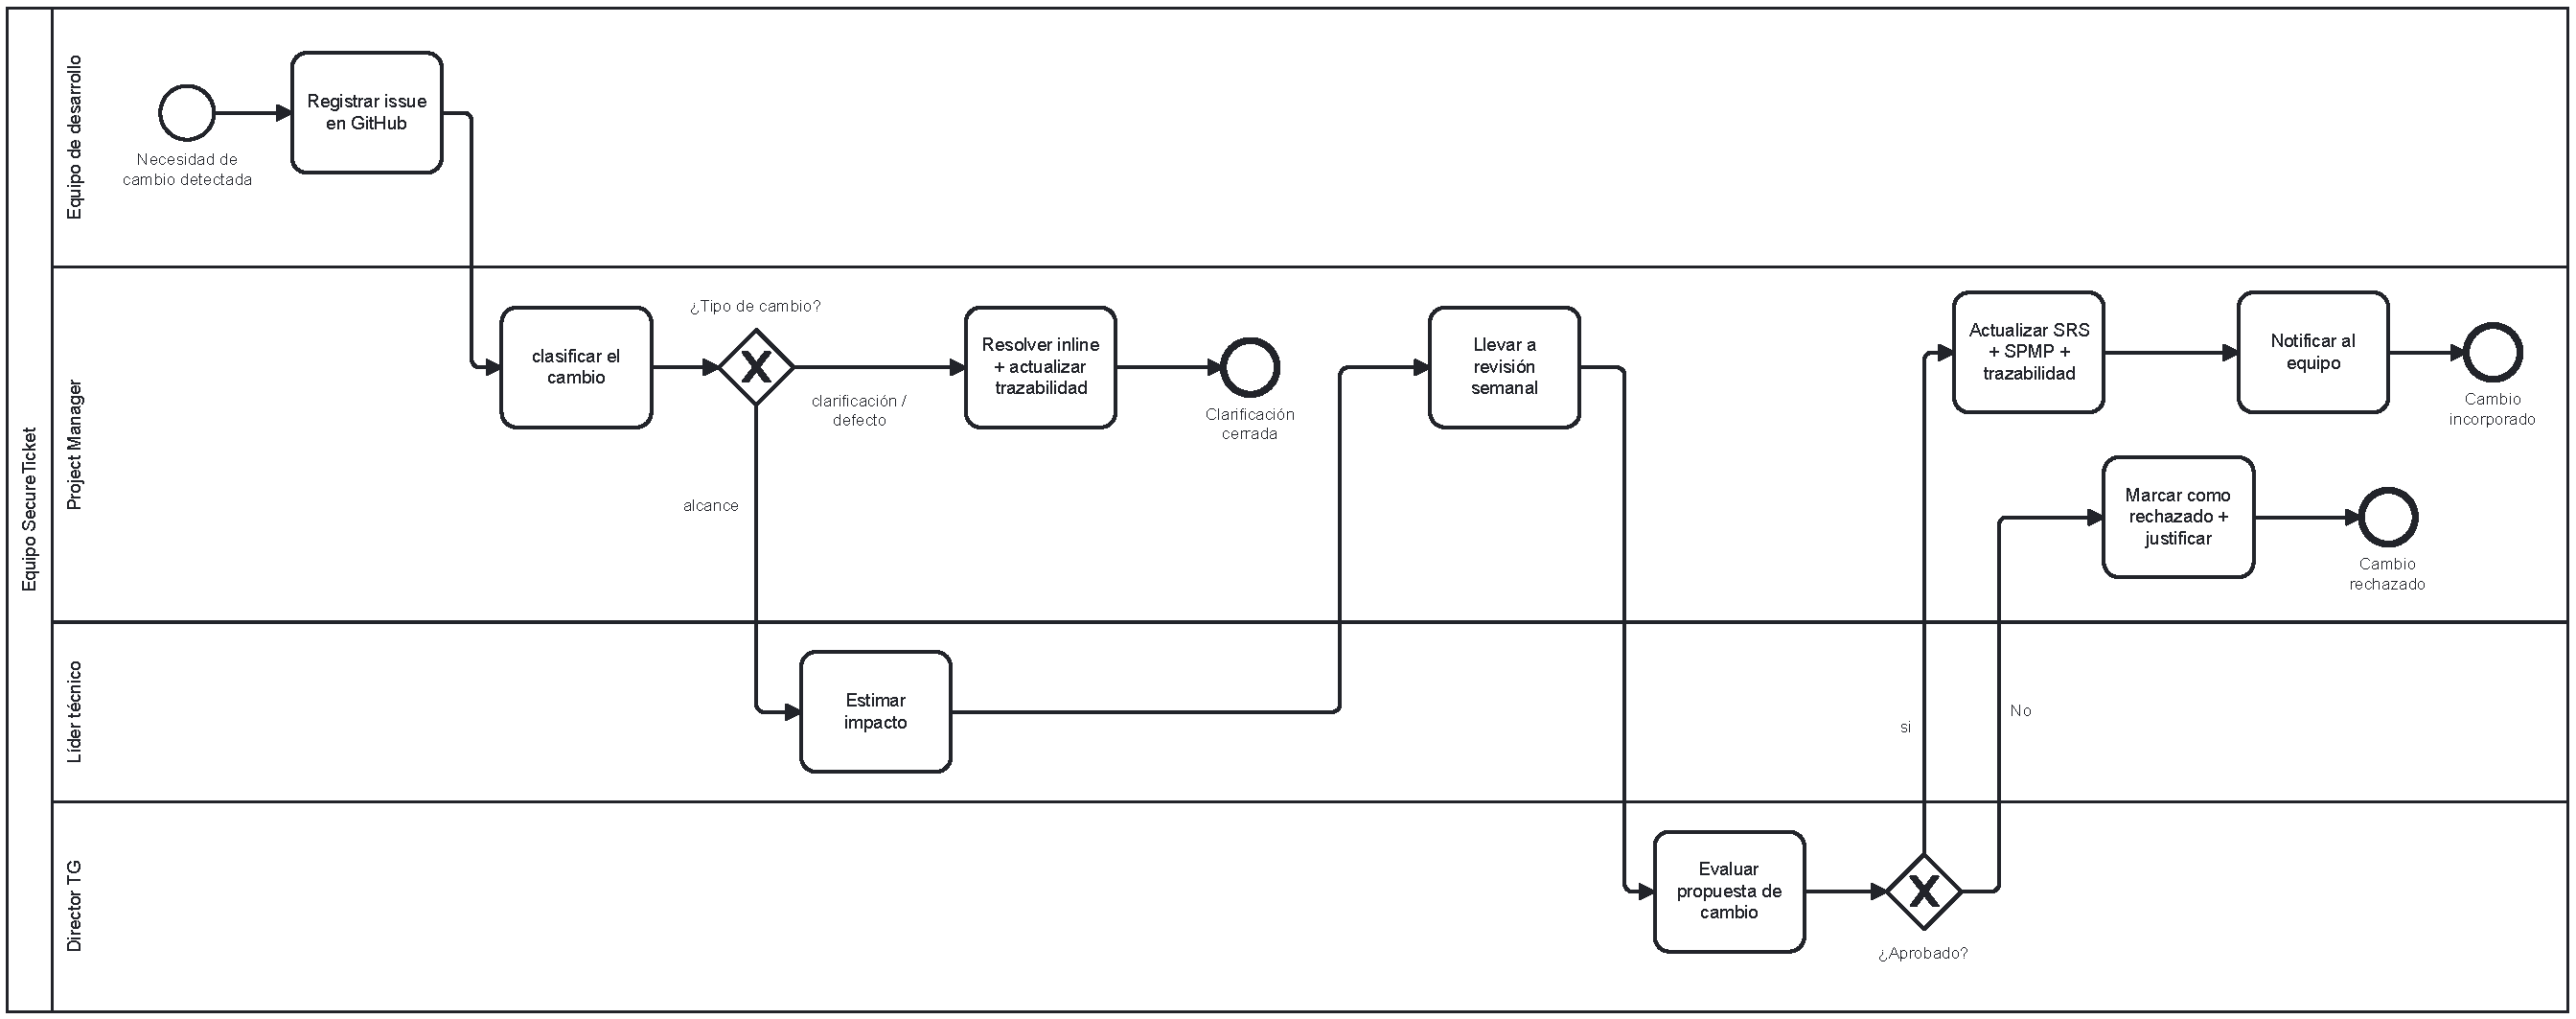
\includegraphics[width=0.95\linewidth]{diagrams/bpmn-req-mgmt.pdf}
        \caption{Flujo BPMN de administración de requerimientos — detección y control de cambios.}
        \label{fig:bpmn-req-mgmt}
      \end{figure}

      \subsubsection{Origen y trazabilidad de los requerimientos}
      Los requerimientos del sistema se documentaron formalmente en el \textbf{SRS}. Cada requerimiento tiene un identificador único (\texttt{RF-XX} para funcionales, \texttt{RNF-XX} para no funcionales) que se referencia en:
      \begin{itemize}
        \item Los \textit{issues} de GitHub que implementan la funcionalidad.
        \item Los casos de prueba que la validan.
        \item Los diagramas del SDD que la describen.
        \item Las acciones de aceptación con el director.
      \end{itemize}

      Esta trazabilidad bidireccional permitió, en cualquier momento del proyecto, responder a preguntas como ``¿qué pruebas cubren \texttt{RF-07}?'' o ``¿qué requerimiento justifica esta función del contrato?''.

      \subsubsection{Proceso de cambio de requerimientos}
      Durante el semestre se produjeron varios cambios al alcance original; los más relevantes están registrados en el historial de cambios del SRS y del SPMP. El procedimiento aplicado para cada cambio fue:
      \begin{enumerate}
        \item \textbf{Detección:} cualquier integrante o el director identifica un requerimiento ambiguo, faltante o desalineado con la realidad técnica.
        \item \textbf{Propuesta:} se abre un \textit{issue} en GitHub etiquetado como \texttt{scope-change}, con descripción del cambio y motivación.
        \item \textbf{Análisis de impacto:} el PM (Andrés Manosalva) evalúa el impacto en alcance, calendario y presupuesto. Si el impacto es mayor, se consulta al subgrupo técnico afectado.
        \item \textbf{Aprobación:} en la revisión semanal con el director se discute y se aprueba o rechaza el cambio.
        \item \textbf{Registro:} el cambio se documenta en el historial de cambios del SRS, y si afecta planeación, también en el SPMP.
        \item \textbf{Comunicación:} se actualiza el tablero Kanban y se informa al equipo en el canal de Discord correspondiente.
      \end{enumerate}

      \subsubsection{Cambios de alcance materializados}
      Los cambios de alcance más relevantes durante el semestre 2026-1 se resumen en la Tabla~\ref{tab:cambios-alcance}.

      \begin{longtable}{@{}p{2.0cm} p{6.0cm} p{6.6cm}@{}}
        \caption{Cambios de alcance aprobados durante el semestre}
        \label{tab:cambios-alcance}\\
        \toprule
        \textbf{Fecha} & \textbf{Cambio} & \textbf{Motivo / Impacto}\\
        \midrule
        \endfirsthead
        \toprule
        \textbf{Fecha} & \textbf{Cambio} & \textbf{Motivo / Impacto}\\
        \midrule
        \endhead
        \bottomrule
        \endfoot
        Mar.~2026 & Reemplazo de NestJS por Express en el backend & Curva de aprendizaje de NestJS demasiado alta para el tiempo disponible; Express ofrecía la flexibilidad necesaria con menor sobrecarga. Sin impacto en alcance funcional.\\
        Abr.~2026 & Eliminación del modo de verificación \textit{offline} en puerta & Complejidad de implementación (sincronización al volver \textit{online}) no justificada en alcance académico. Liberó $\sim$15 h-persona reasignadas a Phase 4.\\
        Abr.~2026 & Incorporación de Phase 4 (panel admin + STAFF) & Necesidad detectada durante pruebas de integración: organizadores requerían gestión visual de eventos y los verificadores necesitaban un rol diferenciado. Aprobado por el director.\\
        Abr.~2026 & Adopción de \texttt{ticket\_nft\_contract} (SEP-41) & Freighter clasificaba los Classic Assets como ``Tokens'' en lugar de ``Collectibles''; SEP-41 corrige la presentación. Añadió un contrato nuevo al alcance.\\
        May.~2026 & Eliminación de Plan de Pruebas, Guía de Despliegue, Manual de Usuario y Póster como entregables formales & Reorganización del paquete documental final a los seis documentos institucionales (Memoria, Plan de Proyecto, SRS, SDD, Propuesta, Formato de Biblioteca). La información se consolidó en la Memoria de TG.\\
      \end{longtable}

    \subsection{Monitoreo y control de progreso}
    \label{subsec:monitoreo-progreso}

      \subsubsection{Ciclo de monitoreo}
      El monitoreo siguió un \textbf{ciclo semanal sincrónico} respaldado por una \textbf{observación diaria asíncrona}:
      \begin{itemize}
        \item \textbf{Diario (asíncrono):} cada integrante actualiza el estado de sus tareas en el tablero Kanban antes de las 22:00 y envía un breve mensaje en el canal de WhatsApp con avances y bloqueos.
        \item \textbf{Semanal (sincrónico):} reunión de 45--60 min con el director donde se revisan métricas, riesgos y entregables; reunión interna del equipo de 30 min para planear la semana siguiente.
        \item \textbf{Fin de fase:} sesión de cierre donde se valida el cumplimiento de los objetivos de la fase y se levantan lecciones aprendidas.
      \end{itemize}

      \subsubsection{KPIs definidos y resultados}
      Se definieron \textbf{siete KPIs} principales para monitorear avance, calidad y salud del proyecto. La Tabla~\ref{tab:kpis} consolida el indicador, su umbral objetivo y el valor real al cierre del semestre.

      \begin{longtable}{@{}p{5.2cm} p{3.6cm} p{2.8cm} p{2.5cm}@{}}
        \caption{KPIs del proyecto: definición, umbral y resultado final}
        \label{tab:kpis}\\
        \toprule
        \textbf{KPI} & \textbf{Fórmula} & \textbf{Umbral} & \textbf{Resultado}\\
        \midrule
        \endfirsthead
        \toprule
        \textbf{KPI} & \textbf{Fórmula} & \textbf{Umbral} & \textbf{Resultado}\\
        \midrule
        \endhead
        \bottomrule
        \endfoot
        \% de pruebas aprobadas (contratos) & pruebas OK / total & $\geq 95\%$ & \textbf{100\% (58/58)}\\
        \% de cobertura de funciones públicas con pruebas & funciones cubiertas / públicas & $\geq 90\%$ & \textbf{100\%}\\
        Eventos desplegados en \textit{testnet} & eventos desplegados / planificados & $\geq 80\%$ & \textbf{12/12 (100\%)}\\
        Defectos críticos abiertos al cierre & conteo absoluto & $0$ & \textbf{0}\\
        Hitos cumplidos en fecha & hitos a tiempo / total & $\geq 80\%$ & \textbf{8/9 (89\%)}\\
        Cumplimiento de revisiones semanales con director & realizadas / planificadas & $\geq 85\%$ & \textbf{15/16 (94\%)}\\
        Desviación de horas-persona (real vs. estimado) & $|\mathrm{real}-\mathrm{est.}|/\mathrm{est.}$ & $\leq 20\%$ & \textbf{$\sim 10\%$}\\
      \end{longtable}

      \textbf{Notas sobre los KPIs:}
      \begin{itemize}
        \item Las 58 pruebas corresponden a 35 de \texttt{event\_contract} + 13 de \texttt{factory\_contract} + 10 de \texttt{ticket\_nft\_contract}.
        \item El único hito que se desplazó fue ``Backend + Indexer'' (planeado sem.~7--10, ejecutado sem.~7--11 por la curva de aprendizaje con Prisma + Stellar SDK), lo que no afectó hitos posteriores.
        \item La revisión semanal pendiente correspondió a la semana de receso académico de Semana Santa.
      \end{itemize}

      \subsubsection{Métricas auxiliares de seguimiento}
      Además de los KPIs principales, se monitorearon métricas operativas obtenidas del repositorio Git y del tablero Kanban:
      \begin{itemize}
        \item \textbf{\textit{Lead time} promedio} de una tarjeta Kanban (desde \textit{In Progress} hasta \textit{Done}): $\sim 3$ días.
        \item \textbf{\textit{Cycle time} promedio} de un \textit{pull request} (apertura $\rightarrow$ \textit{merge}): $\sim 1{,}5$ días.
        \item \textbf{Tasa de \textit{pull requests} con observaciones} en revisión: $\sim 60\%$, lo que indica que la revisión por pares fue efectiva (no era un ``rubber stamp'').
        \item \textbf{Frecuencia de \textit{commits}} en \texttt{main}: pico en semanas 7--12 (desarrollo intensivo), caída controlada en semanas 15--16 (consolidación documental).
      \end{itemize}

      \subsubsection{Acciones correctivas aplicadas}
      Cuando las métricas o los riesgos indicaban una desviación, se aplicaron acciones correctivas durante el semestre. Las más relevantes:
      \begin{itemize}
        \item \textbf{Semana 4:} la curva de aprendizaje de Soroban era más alta de lo estimado. \textbf{Acción:} se programó una sesión de \textit{pair programming} entre Santiago y Andrés para acelerar el dominio del SDK y se ajustaron las estimaciones del paquete WBS de contratos.
        \item \textbf{Semana 7:} el \textit{target} \texttt{wasm32-unknown-unknown} producía WASMs rechazados por la red. \textbf{Acción:} migración a \texttt{wasm32v1-none}, documentación interna del cambio y actualización del \textit{script} de \textit{build}.
        \item \textbf{Semana 11:} aparecieron desviaciones en el indexer (eventos on-chain no se reflejaban a tiempo en PostgreSQL). \textbf{Acción:} se redujo el intervalo de \textit{polling} de 10 s a 5 s y se añadió manejo de reintentos.
        \item \textbf{Semana 13:} riesgo de Phase 4 (panel admin) consumiendo tiempo de documentación. \textbf{Acción:} reasignación temporal de Juan Diego al frontend de Phase 4 y \textit{freeze} del alcance del panel.
        \item \textbf{Semana 15:} densidad de documentación pendiente. \textbf{Acción:} reuniones diarias breves del equipo (15 min) hasta la entrega final para coordinar cierre de SRS, SDD, Memoria y SPMP en paralelo.
      \end{itemize}

    \subsection{Cierre del Proyecto}
    \label{subsec:cierre-proyecto}

      \subsubsection{Criterios de cierre}
      Para considerar una fase incremental como \textbf{cerrada} se debían cumplir simultáneamente los siguientes criterios:
      \begin{enumerate}
        \item Todos los entregables planificados para la fase están \textit{merged} en \texttt{main} y desplegados (cuando aplica).
        \item Las pruebas asociadas pasan al $100\%$.
        \item No quedan defectos críticos abiertos asociados al alcance de la fase.
        \item El director ha validado el avance en la revisión semanal correspondiente.
        \item Los artefactos académicos afectados (SRS, SDD, SPMP) están actualizados.
      \end{enumerate}

      \subsubsection{Ritual de cierre de fase}
      Al cumplir los criterios anteriores, el equipo ejecutaba un ritual de cierre breve (30--45 min) compuesto por cuatro pasos:
      \begin{enumerate}
        \item \textbf{Demostración:} el líder de la fase muestra el avance funcional a todo el equipo.
        \item \textbf{Revisión de métricas:} se actualizan los KPIs de la Sección~\ref{subsec:monitoreo-progreso} y se contrasta con los umbrales.
        \item \textbf{Lecciones aprendidas:} cada integrante aporta un ``qué funcionó'' y un ``qué mejorar''.
        \item \textbf{Planeación de la siguiente fase:} el PM ajusta el tablero Kanban y reorganiza prioridades según los aprendizajes.
      \end{enumerate}

      \subsubsection{Lecciones aprendidas consolidadas}
      Las lecciones aprendidas más relevantes, extraídas de los cierres de fase y consolidadas para el cierre final del proyecto, son:
      \begin{itemize}
        \item \textbf{Capacitarse antes de planear con detalle.} Las primeras estimaciones sobre Soroban estuvieron infladas por desconocimiento; haber dedicado las semanas 1--2 a entrenamiento ahorró tiempo en fases posteriores.
        \item \textbf{La documentación oficial no siempre coincide con el comportamiento real.} Varios problemas (\textit{target} WASM, reference-types, deploy con \textit{salt}) sólo aparecieron al hacer el primer despliegue real.
        \item \textbf{El indexer es el ``pegamento'' entre Web2 y Web3} y merece la misma atención de pruebas que los contratos.
        \item \textbf{Freezing del alcance al final.} Decidir \textit{freezear} Phase 4 en semana 13 y dedicar las últimas semanas a estabilizar y documentar fue una decisión acertada.
        \item \textbf{Las revisiones semanales con el director fueron el mejor mecanismo de control.} Mantener la cadencia (incluso cuando el avance era modesto) evitó sorpresas en la sustentación.
        \item \textbf{Mantener la documentación al día desde el inicio} es más barato que dejarla para el final; aún así, el equipo necesitó una recta final intensa, lo que indica que el balance puede mejorarse en proyectos futuros.
      \end{itemize}

      \subsubsection{Cierre formal del proyecto}
      El cierre formal del proyecto se llevó a cabo en \textbf{semana 16}, con tres actividades:
      \begin{enumerate}
        \item Entrega de los seis documentos académicos a la coordinación, en formato PDF, el \textbf{24 de mayo de 2026}.
        \item Sustentación pública ante director y jurados en una fecha asignada por la coordinación dentro de la ventana \textbf{25 de mayo -- 5 de junio de 2026}.
        \item Reunión interna de \textit{post-mortem} del equipo: validación de cumplimiento de objetivos, revisión final de métricas, archivo del repositorio y documentación de la versión final v1.5 de este SPMP.
      \end{enumerate}

      \subsubsection{Balance final y cumplimiento de objetivos}
      Al cierre del semestre 2026-1, \projectname{} se entrega como un \textbf{prototipo Web2.5 funcional desplegado en \textit{testnet}} con los tres contratos Soroban operativos, 12 eventos desplegados, backend con indexer, frontend con Freighter y panel administrativo (Phase 4). El balance final se resume en: 100\% de los objetivos comprometidos (más Phase 4 no contemplada inicialmente), 58/58 pruebas aprobadas, 0 defectos críticos abiertos, 8/9 hitos en fecha y presupuesto ejecutado dentro de lo planificado. La Tabla~\ref{tab:cumplimiento-objetivos} consolida el cumplimiento de los objetivos del proyecto.

      \begin{longtable}{@{}p{8.5cm} p{2.2cm} p{4.0cm}@{}}
        \caption{Cumplimiento de objetivos del proyecto}
        \label{tab:cumplimiento-objetivos}\\
        \toprule
        \textbf{Objetivo} & \textbf{Estado} & \textbf{Evidencia}\\
        \midrule
        \endfirsthead
        \toprule
        \textbf{Objetivo} & \textbf{Estado} & \textbf{Evidencia}\\
        \midrule
        \endhead
        \bottomrule
        \endfoot
        Diseñar una arquitectura Web2.5 que combine experiencia Web2 tradicional con NFT opcional. & Cumplido & SDD, vistas C4 y demo E2E.\\
        Implementar tres contratos Soroban (evento, factoría, NFT SEP-41) con pruebas unitarias. & Cumplido & 58/58 pruebas; código en \texttt{main}.\\
        Construir un backend con patrón XDR proxy \textit{stateless} (sin custodia de llaves). & Cumplido & Backend Express + Prisma; auditoría de no-custodia.\\
        Construir un frontend integrado con Freighter Wallet y catálogo Web2. & Cumplido & Frontend React/Vite desplegado en Vercel.\\
        Implementar reventa atómica P2P (\textit{burn/remint}) con comisiones organizador + plataforma. & Cumplido & Flujo E2E ejecutado en \textit{testnet}.\\
        Implementar verificación \textit{on-chain} en puerta vía rol STAFF/Verificador. & Cumplido & Phase 4; demo de redención.\\
        Documentar el trabajo de grado conforme a los estándares académicos de la PUJ. & Cumplido & Seis documentos entregados y validados.\\
        Desplegar al menos 8 eventos de prueba en \textit{testnet}. & Superado & 12/12 eventos desplegados.\\
      \end{longtable}

  % =========================================================
  % SECCIÓN 11 — Entrega del producto
  % =========================================================
  \section{Entrega del producto}
  \label{sec:entrega-producto}

    Esta sección describe el \textbf{plan de transición} mediante el cual el equipo entrega formalmente el producto y la documentación del trabajo de grado a la Pontificia Universidad Javeriana. Dado que \textbf{\projectname} es un prototipo académico (no un producto comercial), el plan de transición se centra en la entrega documental, el acceso al código fuente y la presentación del sistema ante el director y los jurados.

    \subsection{Estrategia de entrega}
    \label{subsec:estrategia-entrega}

      El equipo definió una estrategia de entrega \textbf{en una sola fase consolidada}, sin pilotos previos ni despliegues escalonados, por tratarse de un trabajo de grado con una fecha única de entrega documental: el \textbf{24 de mayo de 2026}. La sustentación se realiza posteriormente, en una fecha asignada por la coordinación dentro de la ventana \textbf{25 de mayo -- 5 de junio de 2026} (por confirmar). La estrategia se apoya en tres pilares:
      \begin{itemize}
        \item \textbf{Entrega documental} del paquete de seis documentos académicos en formato PDF.
        \item \textbf{Entrega del código fuente} mediante enlaces públicos al repositorio Git que aloja el sistema (contratos, backend y frontend), sin transferir el código como archivo descargable.
        \item \textbf{Demostración funcional} del prototipo desplegado en \textit{testnet} ante el director y los jurados, en vivo o como video grabado del recorrido.
      \end{itemize}

      No se contempla una entrega a un cliente comercial ni un despliegue en \textit{mainnet}; el receptor del producto es \textbf{la Universidad} (director, jurados y biblioteca institucional).

    \subsection{Artefactos a entregar}
    \label{subsec:artefactos-entrega}

      La Tabla~\ref{tab:artefactos-entrega} consolida todos los artefactos del paquete final, su formato y su responsable de entrega.

      \begin{longtable}{@{}p{4.5cm} p{4.0cm} p{3.0cm} p{3.0cm}@{}}
        \caption{Artefactos del paquete de entrega final}
        \label{tab:artefactos-entrega}\\
        \toprule
        \textbf{Artefacto} & \textbf{Descripción} & \textbf{Formato} & \textbf{Responsable}\\
        \midrule
        \endfirsthead
        \toprule
        \textbf{Artefacto} & \textbf{Descripción} & \textbf{Formato} & \textbf{Responsable}\\
        \midrule
        \endhead
        \bottomrule
        \endfoot
        Memoria de TG & Documento principal del trabajo de grado & PDF (\LaTeX) & Todos\\
        Plan de Proyecto (SPMP v1.5) & Este documento & PDF (\LaTeX) & Todos\\
        SRS & Especificación de Requisitos de Software & PDF (\LaTeX) & Todos\\
        SDD & Especificación del Diseño (vistas C4, secuencias, datos) & PDF (\LaTeX) & Todos\\
        Propuesta de TG & Anteproyecto aprobado & PDF & Todos\\
        Formato de Biblioteca & Formato institucional para entrega del TG & PDF & Todos\\
        Enlace al repositorio Git & Código fuente (contratos, backend, frontend) & URL pública & Todos\\
        Direcciones de contratos en \textit{testnet} & WASM hashes y direcciones de 12 eventos desplegados & Lista en Memoria de TG & Blockchain (Santiago Mesa)\\
        Demo final & Sistema en \textit{testnet} en vivo o video grabado & Demo/MP4 & Todos\\
      \end{longtable}

      \textbf{Aclaraciones:}
      \begin{itemize}
        \item Sólo los \textbf{seis documentos} (Memoria, Plan de Proyecto, SRS, SDD, Propuesta y Formato de Biblioteca) se entregan formalmente a la coordinación académica.
        \item El \textbf{código fuente} no se anexa al paquete documental; sólo se entregan los enlaces públicos al repositorio.
        \item El \textbf{Demo final} no se anexa como artefacto descargable; se presenta el día de la sustentación.
      \end{itemize}

    \subsection{Cronograma de entrega}
    \label{subsec:cronograma-entrega}

      El cronograma de la entrega final, ejecutado durante las dos últimas semanas del semestre, se resume en la Tabla~\ref{tab:cronograma-entrega}.

      \begin{longtable}{@{}p{3.0cm} p{8.5cm} p{3.0cm}@{}}
        \caption{Cronograma de entrega final}
        \label{tab:cronograma-entrega}\\
        \toprule
        \textbf{Fecha (2026)} & \textbf{Actividad} & \textbf{Responsable}\\
        \midrule
        \endfirsthead
        \toprule
        \textbf{Fecha (2026)} & \textbf{Actividad} & \textbf{Responsable}\\
        \midrule
        \endhead
        \bottomrule
        \endfoot
        11 -- 15 may & Consolidación final de los seis documentos; revisiones cruzadas entre integrantes & Todos\\
        15 may & Compilación final de PDFs y revisión de consistencia entre documentos & PM\\
        16 may & Despliegue final estable de los 12 eventos en \textit{testnet}; verificación E2E del prototipo & QA/DevOps + Blockchain\\
        17 may & Revisión final con el director (validación de paquete documental) & PM + Director\\
        18 -- 22 may & Aplicación de observaciones del director; grabación del video del demo (respaldo en caso de fallo durante la sustentación); ensayos de la sustentación & Todos\\
        \textbf{24 may} & \textbf{Entrega del paquete documental (seis PDFs) a coordinación académica --- cierre del proyecto} & Todos\\
        25 may -- 5 jun & Ventana de sustentación ante director y jurados (fecha exacta asignada por la coordinación) & Todos\\
        Posterior a la sustentación & Atención a observaciones de los jurados y subida de versión final al repositorio institucional & Todos\\
      \end{longtable}

    \subsection{Capacitación y soporte al receptor}
    \label{subsec:capacitacion-soporte}

      Por la naturaleza académica del proyecto, la capacitación al receptor (jurados y director) se limita a la presentación durante la sustentación y al material documental.

      \subsubsection{Capacitación durante la sustentación}
      \begin{itemize}
        \item \textbf{Presentación expositiva} ($\sim 20$ min): contexto, problema, propuesta arquitectónica, decisiones clave y resultados.
        \item \textbf{Demostración funcional} ($\sim 10$ min): recorrido E2E del prototipo en \textit{testnet} mostrando los flujos principales (compra Web2, asegurar en blockchain, reventa P2P, verificación en puerta).
        \item \textbf{Sesión de preguntas} ($\sim 15$ min): respuesta a inquietudes técnicas y de gestión del trabajo de grado.
      \end{itemize}

      \subsubsection{Material de apoyo}
      Los jurados disponen, previo a la sustentación, del \textbf{paquete documental completo} (seis documentos) para revisión. Durante la sustentación, el equipo atiende los materiales adicionales que los jurados soliciten en ese momento (por ejemplo, enlaces al repositorio, direcciones de contratos en \textit{testnet} o URLs del prototipo desplegado), sin que el equipo se comprometa de antemano a entregar ninguno de ellos como parte obligatoria del paquete.

      \subsubsection{Soporte post-entrega}
      Tras la sustentación, el equipo asume el siguiente compromiso de soporte:
      \begin{itemize}
        \item \textbf{Atención de observaciones de los jurados:} si los jurados solicitan correcciones o ajustes menores en los documentos, el equipo los aplica dentro del plazo establecido por la coordinación académica.
        \item \textbf{Disponibilidad del prototipo en \textit{testnet}:} el frontend, backend e indexer permanecen desplegados al menos hasta el cierre formal del semestre.
        \item \textbf{Repositorio Git:} permanece público para consulta, sin compromiso de mantenimiento ni evolución.
      \end{itemize}

      \textbf{Importante:} el equipo \textbf{no asume responsabilidad de mantenimiento, evolución funcional ni operación} del prototipo después del cierre del semestre. La transferencia es un \textit{snapshot} académico, no una entrega operativa.

    \subsection{Criterios de aceptación de la entrega}
    \label{subsec:aceptacion-entrega}

      La entrega se considera \textbf{aceptada y cerrada} cuando se cumplen simultáneamente las siguientes condiciones:
      \begin{enumerate}
        \item Los seis documentos académicos están entregados a la coordinación en formato PDF y firmados (cuando aplica) por el director.
        \item La sustentación ha sido presentada ante director y jurados en la fecha asignada por la coordinación dentro de la ventana 25 de mayo -- 5 de junio de 2026.
        \item Los jurados emiten su calificación / acta de sustentación según los lineamientos institucionales.
        \item Las observaciones de los jurados (si las hubiera) están atendidas y los documentos finales actualizados son subidos al repositorio institucional de la Universidad.
      \end{enumerate}

      A partir del cumplimiento de estas condiciones, el proyecto \textbf{\projectname} se considera formalmente \textbf{transferido} a la Universidad como parte del trabajo de grado del Grupo 12.

  % =========================================================
  % SECCIÓN 12 — Procesos de soporte
  % =========================================================
  \section{Procesos de soporte}
  \label{sec:procesos-soporte}

    Esta sección documenta los \textbf{procesos transversales} que apoyaron la ejecución del proyecto: el ambiente de trabajo y las reglas internas del equipo, el análisis y la administración de riesgos, la gestión de configuración y documentación, las métricas del proceso y el control de calidad.

    \subsection{Ambiente de trabajo y reglas del equipo}
    \label{subsec:ambiente-equipo}

      \subsubsection{Ambiente de trabajo}
      El equipo trabajó en una modalidad \textbf{predominantemente remota} desde las residencias de cada integrante, con reuniones presenciales puntuales (revisiones con el director, sesiones de \textit{pair programming} en momentos críticos y ensayos de la sustentación). El ambiente técnico unificado se aseguró mediante un archivo \texttt{SETUP.md} en el repositorio con las versiones exigidas de Rust, Node, soroban-cli y demás dependencias.

      \subsubsection{Reglas del equipo}
      Las reglas internas del equipo, acordadas en la primera semana del semestre y mantenidas durante todo el proyecto, son:
      \begin{itemize}
        \item \textbf{Respeto y diálogo constructivo:} cualquier discrepancia técnica o de gestión se discute en el canal correspondiente; no se permiten descalificaciones personales.
        \item \textbf{Asistencia a reuniones semanales con el director} como prioridad alta; ausencias sólo por causas justificadas y con aviso previo.
        \item \textbf{Asistencia a reuniones internas del equipo} con la misma prioridad que las académicas.
        \item \textbf{Compromiso con las tareas asignadas:} si un integrante anticipa que no podrá cumplir una entrega, lo comunica con al menos 48 h de antelación para reasignar o ajustar prioridades.
        \item \textbf{Revisión por pares obligatoria} en todo \textit{pull request} antes de \textit{merge} a \texttt{main}.
        \item \textbf{No \textit{push} directo a \texttt{main}:} todo cambio pasa por rama y \textit{pull request}.
        \item \textbf{Mantener la documentación al día} con cada cambio funcional relevante.
        \item \textbf{Confidencialidad de credenciales:} secretos en archivos \texttt{.env} \textit{gitignored}; nunca se publican en repositorios o canales abiertos.
        \item \textbf{Decisiones por consenso} en reuniones internas; el PM resuelve empates cuando es necesario.
      \end{itemize}

    \subsection{Análisis y administración de riesgos}
    \label{subsec:riesgos}

      \subsubsection{Proceso de gestión de riesgos}
      La gestión de riesgos siguió un ciclo continuo de cuatro pasos: \textbf{identificación} (en cualquier momento por cualquier integrante o por el director), \textbf{análisis} (estimación de probabilidad e impacto), \textbf{respuesta} (mitigación, transferencia, aceptación o evitación) y \textbf{monitoreo} (revisión semanal del estado de cada riesgo activo). La Figura~\ref{fig:bpmn-riesgos} formaliza el flujo: el \textbf{Equipo} identifica riesgos nuevos o cambios en cada reunión semanal (\textit{timer start event}); el \textbf{Project Manager} calcula probabilidad × impacto y, si el resultado clasifica el riesgo como crítico (P × I $\geq 12$), define plan de mitigación, responsable y recursos, y monitorea su evolución semanalmente. Los riesgos no críticos quedan en monitoreo pasivo. El registro de riesgos (consolidado en esta sección) se actualiza al final del proceso.

      \begin{figure}[H]
        \centering
        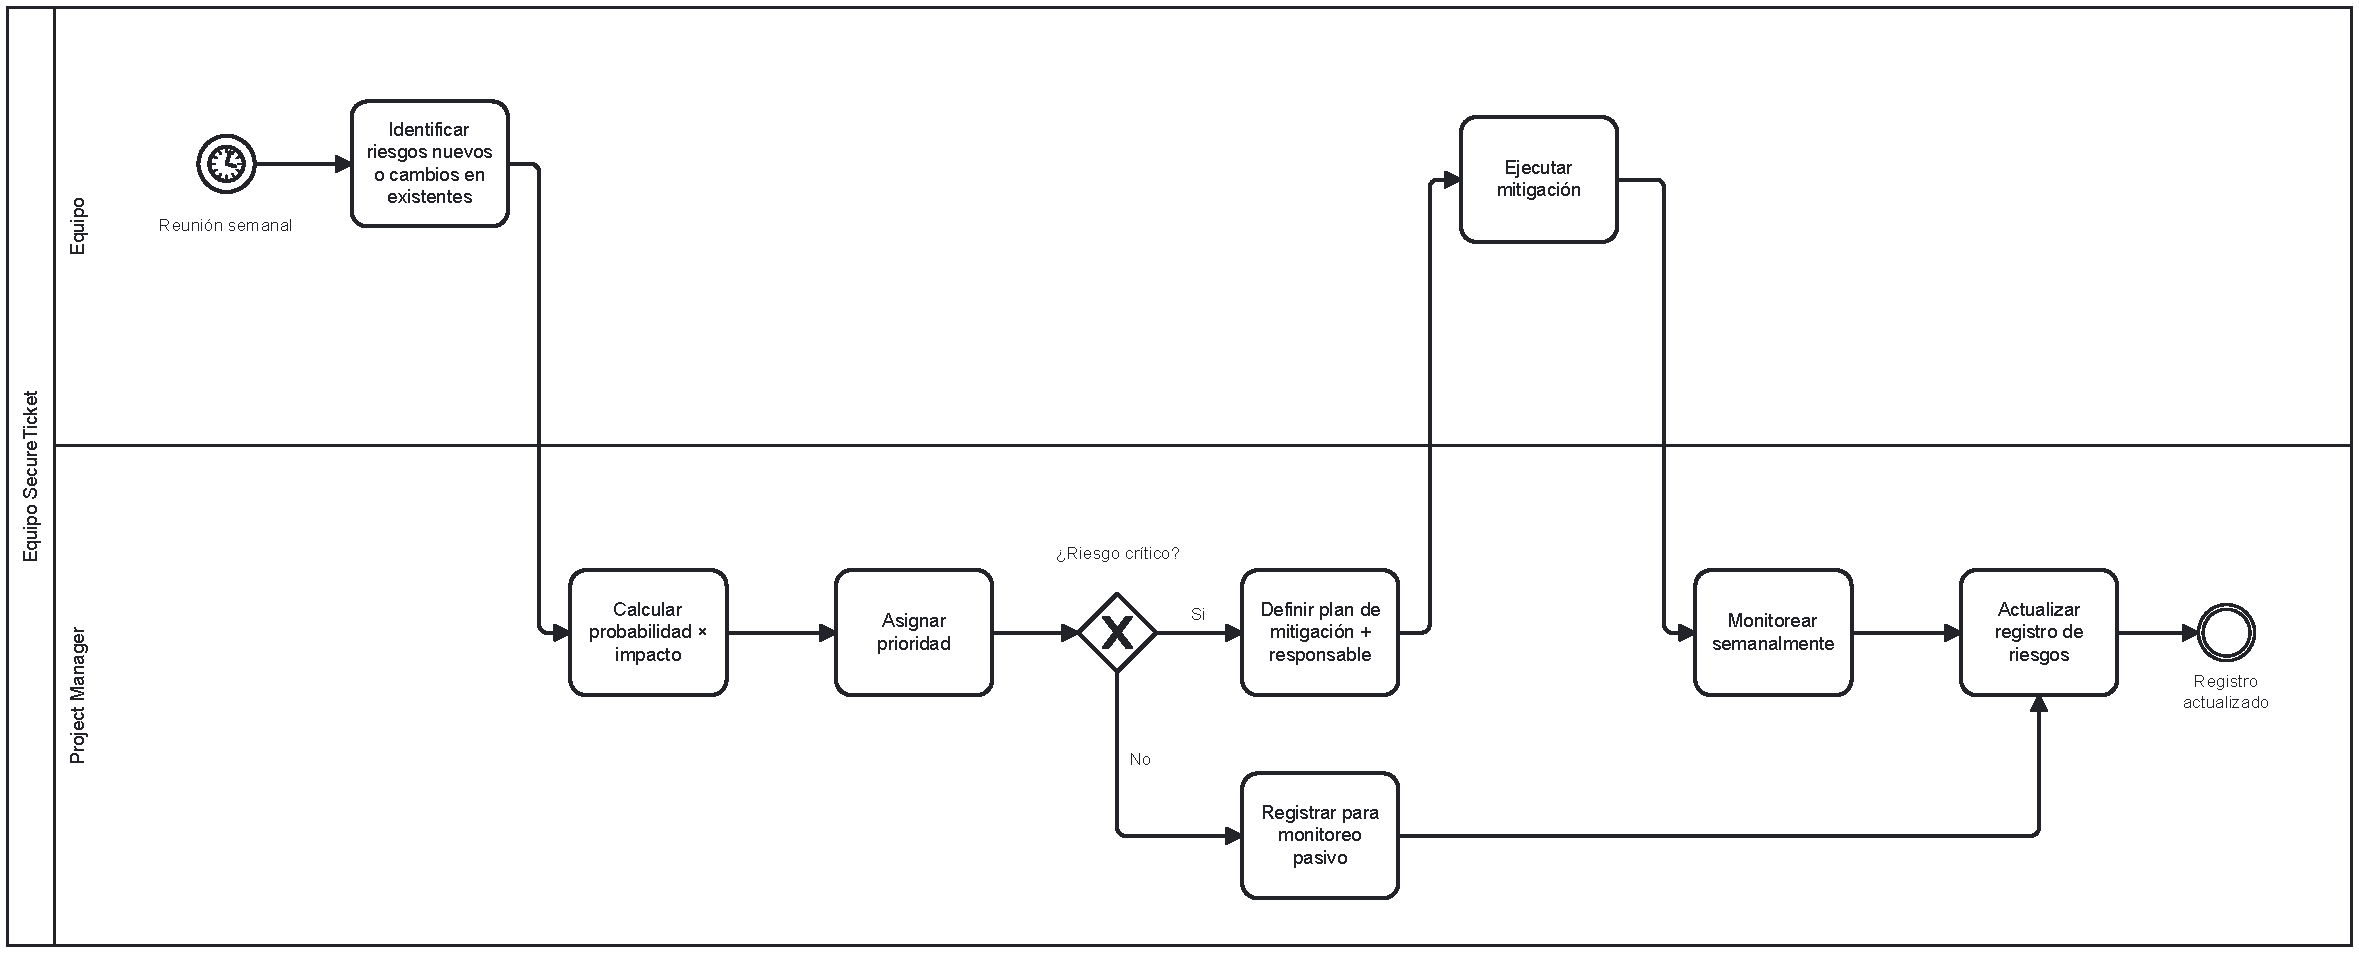
\includegraphics[width=0.85\linewidth]{diagrams/bpmn-riesgos.pdf}
        \caption{Flujo BPMN de gestión de riesgos — identificación, valoración y monitoreo.}
        \label{fig:bpmn-riesgos}
      \end{figure}

      La probabilidad y el impacto se evaluaron en una escala cualitativa de tres niveles (Baja / Media / Alta), y la exposición se calculó como el producto categórico de ambos. Se utilizó la matriz de la Tabla~\ref{tab:matriz-riesgo}.

      \begin{table}[H]
        \centering
        \begin{tabular}{@{}c|ccc@{}}
          \toprule
          \textbf{Probabilidad $\backslash$ Impacto} & \textbf{Bajo} & \textbf{Medio} & \textbf{Alto}\\
          \midrule
          \textbf{Alta}  & Medio & Alto  & Crítico\\
          \textbf{Media} & Bajo  & Medio & Alto\\
          \textbf{Baja}  & Bajo  & Bajo  & Medio\\
          \bottomrule
        \end{tabular}
        \caption{Matriz cualitativa de exposición al riesgo}
        \label{tab:matriz-riesgo}
      \end{table}

      \subsubsection{Registro de riesgos del proyecto}
      La Tabla~\ref{tab:registro-riesgos} consolida los \textbf{principales riesgos identificados} durante el semestre 2026-1, su evaluación inicial, la estrategia de respuesta y el estado al cierre del proyecto.

      \begin{longtable}{@{}p{0.6cm} p{3.8cm} p{1.0cm} p{1.0cm} p{1.0cm} p{4.6cm} p{1.5cm}@{}}
        \caption{Registro de riesgos del proyecto}
        \label{tab:registro-riesgos}\\
        \toprule
        \textbf{ID} & \textbf{Riesgo} & \textbf{Prob.} & \textbf{Imp.} & \textbf{Exp.} & \textbf{Respuesta aplicada} & \textbf{Estado}\\
        \midrule
        \endfirsthead
        \toprule
        \textbf{ID} & \textbf{Riesgo} & \textbf{Prob.} & \textbf{Imp.} & \textbf{Exp.} & \textbf{Respuesta aplicada} & \textbf{Estado}\\
        \midrule
        \endhead
        \bottomrule
        \endfoot
        R1 & Curva de aprendizaje de Soroban más alta de lo estimado & Alta & Alto & Crítico & \textit{Pair programming} en sem.~4; ajuste de estimaciones; documentación interna del SDK & Materializado / Mitigado\\
        R2 & Inestabilidad de la \textit{testnet} de Stellar (\textit{downtimes}, cambios de RPC) & Media & Alto & Alto & Configuración de RPC alterno; reintentos con \textit{backoff} en backend e indexer & Materializado / Mitigado\\
        R3 & Cambios en \texttt{soroban-sdk} durante el semestre & Media & Medio & Medio & Fijar versión SDK en \texttt{Cargo.toml}; documentar incompatibilidades & Materializado / Mitigado\\
        R4 & Pérdida o exposición de llaves privadas de \textit{testnet} & Baja & Alto & Medio & \texttt{.env.deploy} \textit{gitignored}; semillas en gestor local; rotación si se sospecha exposición & No materializado\\
        R5 & Desincronización entre estado on-chain y PostgreSQL & Media & Alto & Alto & Indexer con \textit{polling} cada 5 s; reintentos; mecanismo de reconciliación manual & Materializado / Mitigado\\
        R6 & Indisponibilidad de un integrante por carga académica & Alta & Medio & Alto & Asignación de \textit{back-up} en cada paquete WBS; reasignación temporal en sem.~13 & Materializado / Aceptado\\
        R7 & Cambios de alcance impulsados por revisiones del director & Media & Medio & Medio & Proceso de cambio formal (Sección~\ref{subsec:admin-requerimientos}); evaluación de impacto antes de aceptar & Materializado / Gestionado\\
        R8 & Defectos críticos descubiertos en la recta final & Media & Alto & Alto & \textit{Freeze} de alcance en sem.~13; \textit{focus} de QA en sem.~14--15 & No materializado\\
        R9 & Bloqueo en sustentación por fallo del prototipo en vivo & Media & Alto & Alto & Grabación de video del demo como respaldo & No materializado (mitigado preventivamente)\\
        R10 & Inconsistencias entre documentos académicos (SRS, SDD, SPMP, Memoria) & Alta & Medio & Alto & Revisiones cruzadas en sem.~15; trazabilidad por IDs & Materializado / Mitigado\\
        R11 & Costos de infraestructura inesperados (cuotas excedidas en \textit{free tier}) & Baja & Medio & Bajo & Monitoreo de consumo; contingencia presupuestal del 10\% & No materializado\\
        R12 & Pérdida de datos por borrado accidental del repositorio o base de datos & Baja & Alto & Medio & \textit{Backups} automáticos de Supabase; ramas protegidas en GitHub & No materializado\\
      \end{longtable}

      \subsubsection{Aprendizajes sobre gestión de riesgos}
      Los riesgos \textbf{técnicos relacionados con Soroban} (R1, R2, R3, R5) tuvieron el mayor impacto real y consumieron la mayor parte de las acciones correctivas del proyecto. Los riesgos \textbf{operativos} (R6, R7) se gestionaron de forma rutinaria a través de las reuniones semanales. Los riesgos \textbf{preventivos para la sustentación} (R8, R9) se monitorearon de cerca en las últimas semanas y se mitigaron preventivamente.

    \subsection{Administración de configuración y documentación}
    \label{subsec:gestion-configuracion}

      El proceso de control de cambios sobre los elementos de configuración (CI) se formaliza en la Figura~\ref{fig:bpmn-config-mgmt}. El \textbf{Autor} crea una rama \texttt{feature/*}, hace \textit{commit} con mensaje convencional y abre un \textit{pull request} con descripción, pruebas y tipo de cambio. El \textbf{Revisor} ejecuta \textit{code review} y verifica el estado de CI (\textit{build} + pruebas + \textit{lint}). Solo con aprobación y CI verde el cambio entra al \textbf{Repositorio} \texttt{main}, donde recibe un \textit{tag} de versión semántica. Si el cambio afecta artefactos académicos (SPMP, SRS, SDD), el \textbf{Project Manager} actualiza el Historial de Cambios y la versión del documento.

      \begin{figure}[H]
        \centering
        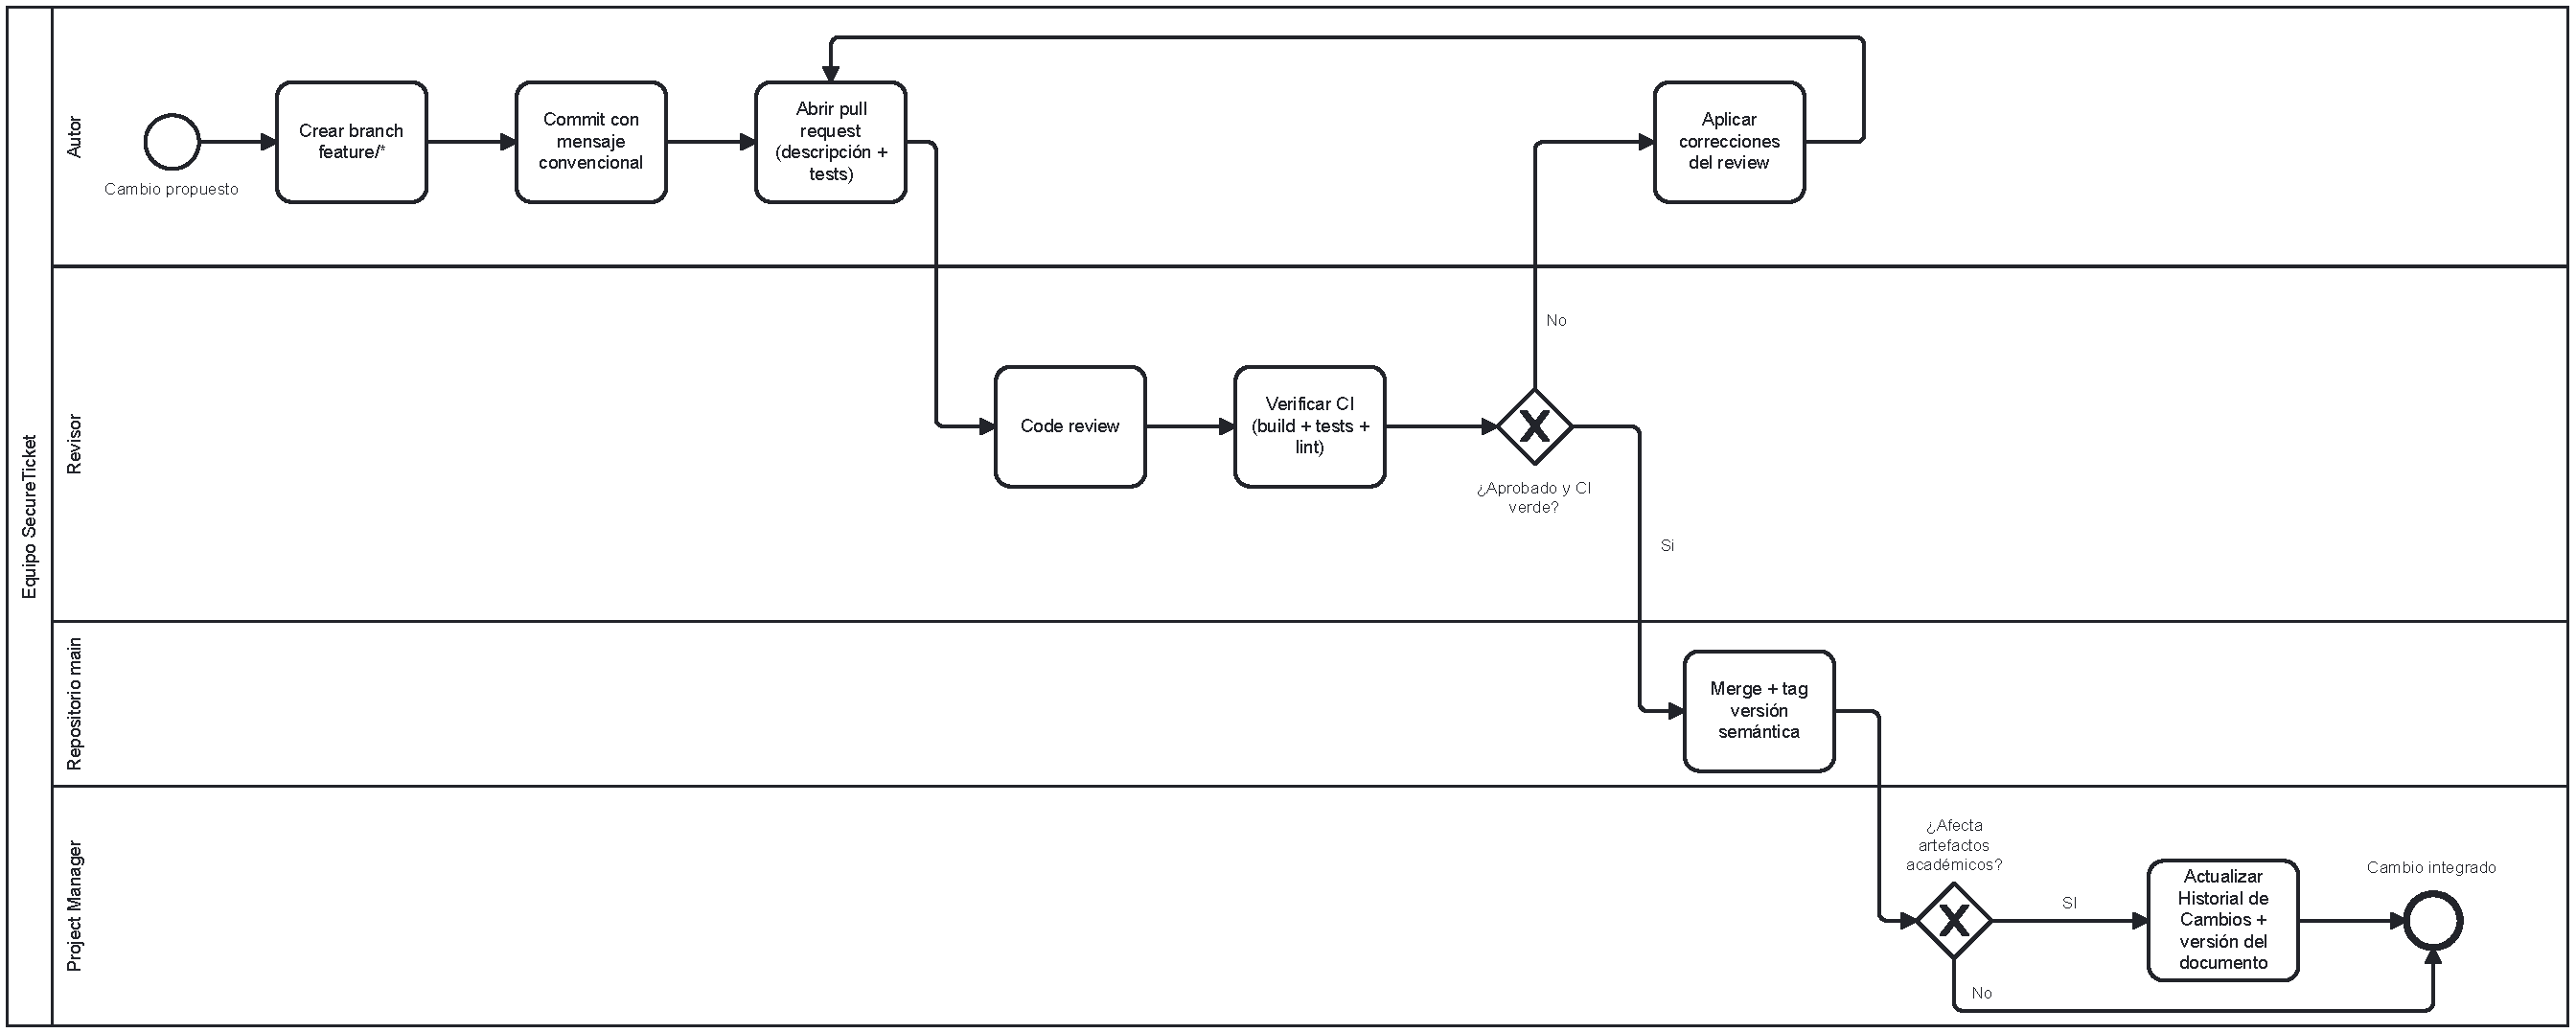
\includegraphics[width=0.95\linewidth]{diagrams/bpmn-config-mgmt.pdf}
        \caption{Flujo BPMN de control de cambios de configuración (pull request, code review, merge y bitácora).}
        \label{fig:bpmn-config-mgmt}
      \end{figure}

      \subsubsection{Identificación de elementos de configuración}
      Los \textbf{elementos de configuración (CI)} del proyecto, sometidos a control formal de versiones, son:
      \begin{itemize}
        \item \textbf{Código fuente:} contratos Rust, backend TypeScript, frontend TypeScript, esquemas Prisma, \textit{scripts} de despliegue.
        \item \textbf{Documentos académicos:} fuentes \LaTeX{} de Memoria de TG, SPMP, SRS, SDD, Propuesta y Formato de Biblioteca, junto con sus imágenes/diagramas.
        \item \textbf{Configuración de infraestructura:} \texttt{.env.example}, \texttt{Cargo.toml}, \texttt{package.json}, archivos de Prisma, archivos de despliegue para Vercel y Railway.
        \item \textbf{Artefactos compilados:} archivos WASM de los contratos y sus \textit{hashes} (no versionados en Git, pero registrados en la documentación).
      \end{itemize}

      \subsubsection{Control de versiones}
      \begin{itemize}
        \item \textbf{Repositorio único} en GitHub bajo la organización \textit{Tesis-Stellar}, con el código y los documentos \LaTeX{} en carpetas separadas.
        \item \textbf{Rama \texttt{main} protegida:} requiere \textit{pull request} aprobado, revisión por pares y CI verde antes de \textit{merge}.
        \item \textbf{Ramas de trabajo} con prefijos por tipo: \texttt{feat/}, \texttt{fix/}, \texttt{docs/}, \texttt{chore/}.
        \item \textbf{Convención de \textit{commits}} basada en \textit{Conventional Commits} (tipo: descripción) para facilitar el rastreo del historial.
        \item \textbf{\textit{Tags} de versión} para hitos significativos del código (no obligatorios).
      \end{itemize}

      \subsubsection{Control de cambios}
      Todo cambio sobre un elemento de configuración sigue el flujo:
      \begin{enumerate}
        \item Creación de \textit{issue} (cuando aplica) con descripción del cambio.
        \item Apertura de rama y desarrollo del cambio.
        \item \textit{Pull request} con descripción, vinculación a \textit{issue} y, cuando aplica, evidencias visuales (capturas, GIFs).
        \item Revisión por al menos un compañero distinto al autor.
        \item Ajustes solicitados (si los hay) y aprobación.
        \item \textit{Merge} a \texttt{main} mediante \textit{squash} o \textit{merge commit} estándar (según política por carpeta).
      \end{enumerate}

      \subsubsection{Gestión de versiones de los documentos}
      \begin{itemize}
        \item Cada documento académico mantiene su propio \textbf{historial de cambios} al inicio del documento, con fecha, descripción y autor.
        \item Los documentos se compilan a PDF localmente con \texttt{pdflatex}; el PDF compilado más reciente se versiona en el repositorio cuando hay una revisión sustancial.
        \item Las versiones de los documentos se sincronizan con los hitos del proyecto (por ejemplo, este SPMP llega a v1.5 al cierre).
      \end{itemize}

      \subsubsection{Respaldos}
      \begin{itemize}
        \item Repositorio replicado en GitHub (servicio externo, redundancia automática).
        \item Supabase realiza \textit{backups} automáticos diarios del esquema PostgreSQL.
        \item Cada integrante mantiene una copia local del repositorio actualizada.
      \end{itemize}

    \subsection{Métricas y proceso de medición}
    \label{subsec:metricas-medicion}

      Esta subsección describe \textbf{cómo} se midió el proyecto. Los \textbf{valores finales} de los KPIs se reportaron en la Sección~\ref{subsec:monitoreo-progreso}.

      \subsubsection{Proceso de medición}
      \begin{enumerate}
        \item \textbf{Definición:} cada KPI cuenta con un nombre, fórmula, umbral y fuente de datos definidos antes de empezar a medirlo.
        \item \textbf{Recolección:} las métricas se recolectan al final de cada semana, con responsable claro (PM para métricas de gestión, líder de subsistema para métricas técnicas).
        \item \textbf{Almacenamiento:} se mantienen en una hoja compartida en Google Drive con histórico por semana.
        \item \textbf{Análisis:} se revisan en la reunión semanal con el director; las desviaciones se discuten y, si aplica, se activan acciones correctivas.
        \item \textbf{Reporte:} la versión consolidada se incorpora a este SPMP y a la Memoria de TG.
      \end{enumerate}

      \subsubsection{Categorías de métricas}
      \begin{itemize}
        \item \textbf{Métricas de progreso:} hitos cumplidos, eventos desplegados, cumplimiento de cronograma.
        \item \textbf{Métricas de calidad:} \% de pruebas aprobadas, cobertura, defectos abiertos, defectos críticos.
        \item \textbf{Métricas de proceso:} \textit{lead time}, \textit{cycle time} de \textit{pull requests}, tasa de \textit{PRs} con observaciones.
        \item \textbf{Métricas de esfuerzo:} desviación de horas-persona estimadas vs. reales.
        \item \textbf{Métricas de colaboración:} asistencia a reuniones semanales, frecuencia de \textit{commits} por integrante.
      \end{itemize}

      \subsubsection{Fuentes de datos}
      \begin{itemize}
        \item \textbf{GitHub:} \textit{commits}, \textit{pull requests}, \textit{issues}, tablero Kanban (GitHub Projects).
        \item \textbf{Suites de prueba:} salida de \texttt{cargo test} (contratos), \texttt{npm test} (backend) y pruebas E2E del frontend.
        \item \textbf{\textit{Block explorer} de Stellar:} verificación del estado de contratos desplegados.
        \item \textbf{Hoja de horas} compartida en Google Drive.
      \end{itemize}

    \subsection{Control de calidad}
    \label{subsec:control-calidad}

      El control de calidad se apoya en tres mecanismos complementarios: \textbf{verificación} (¿lo estamos construyendo bien?), \textbf{validación} (¿estamos construyendo lo correcto?) y \textbf{revisiones} (inspección humana). La Figura~\ref{fig:bpmn-calidad} formaliza el flujo: el \textbf{Desarrollador} arranca tres actividades de verificación en paralelo (\textit{gateway} AND) — \texttt{cargo test}, \texttt{clippy + eslint} y \textit{build}/compilación WASM/TS —; al converger, ejecuta pruebas de integración del backend. Luego, el \textbf{Revisor} hace \textit{code review} y revisión documental; el Desarrollador ejecuta pruebas E2E en \textit{testnet} y el \textbf{Director TG} valida el avance en la revisión semanal. Si la funcionalidad pasa la \textit{Definition of Done} la tarea se marca como DONE y se actualizan métricas; en caso contrario, el defecto se documenta y vuelve al ciclo de integración.

      \begin{figure}[H]
        \centering
        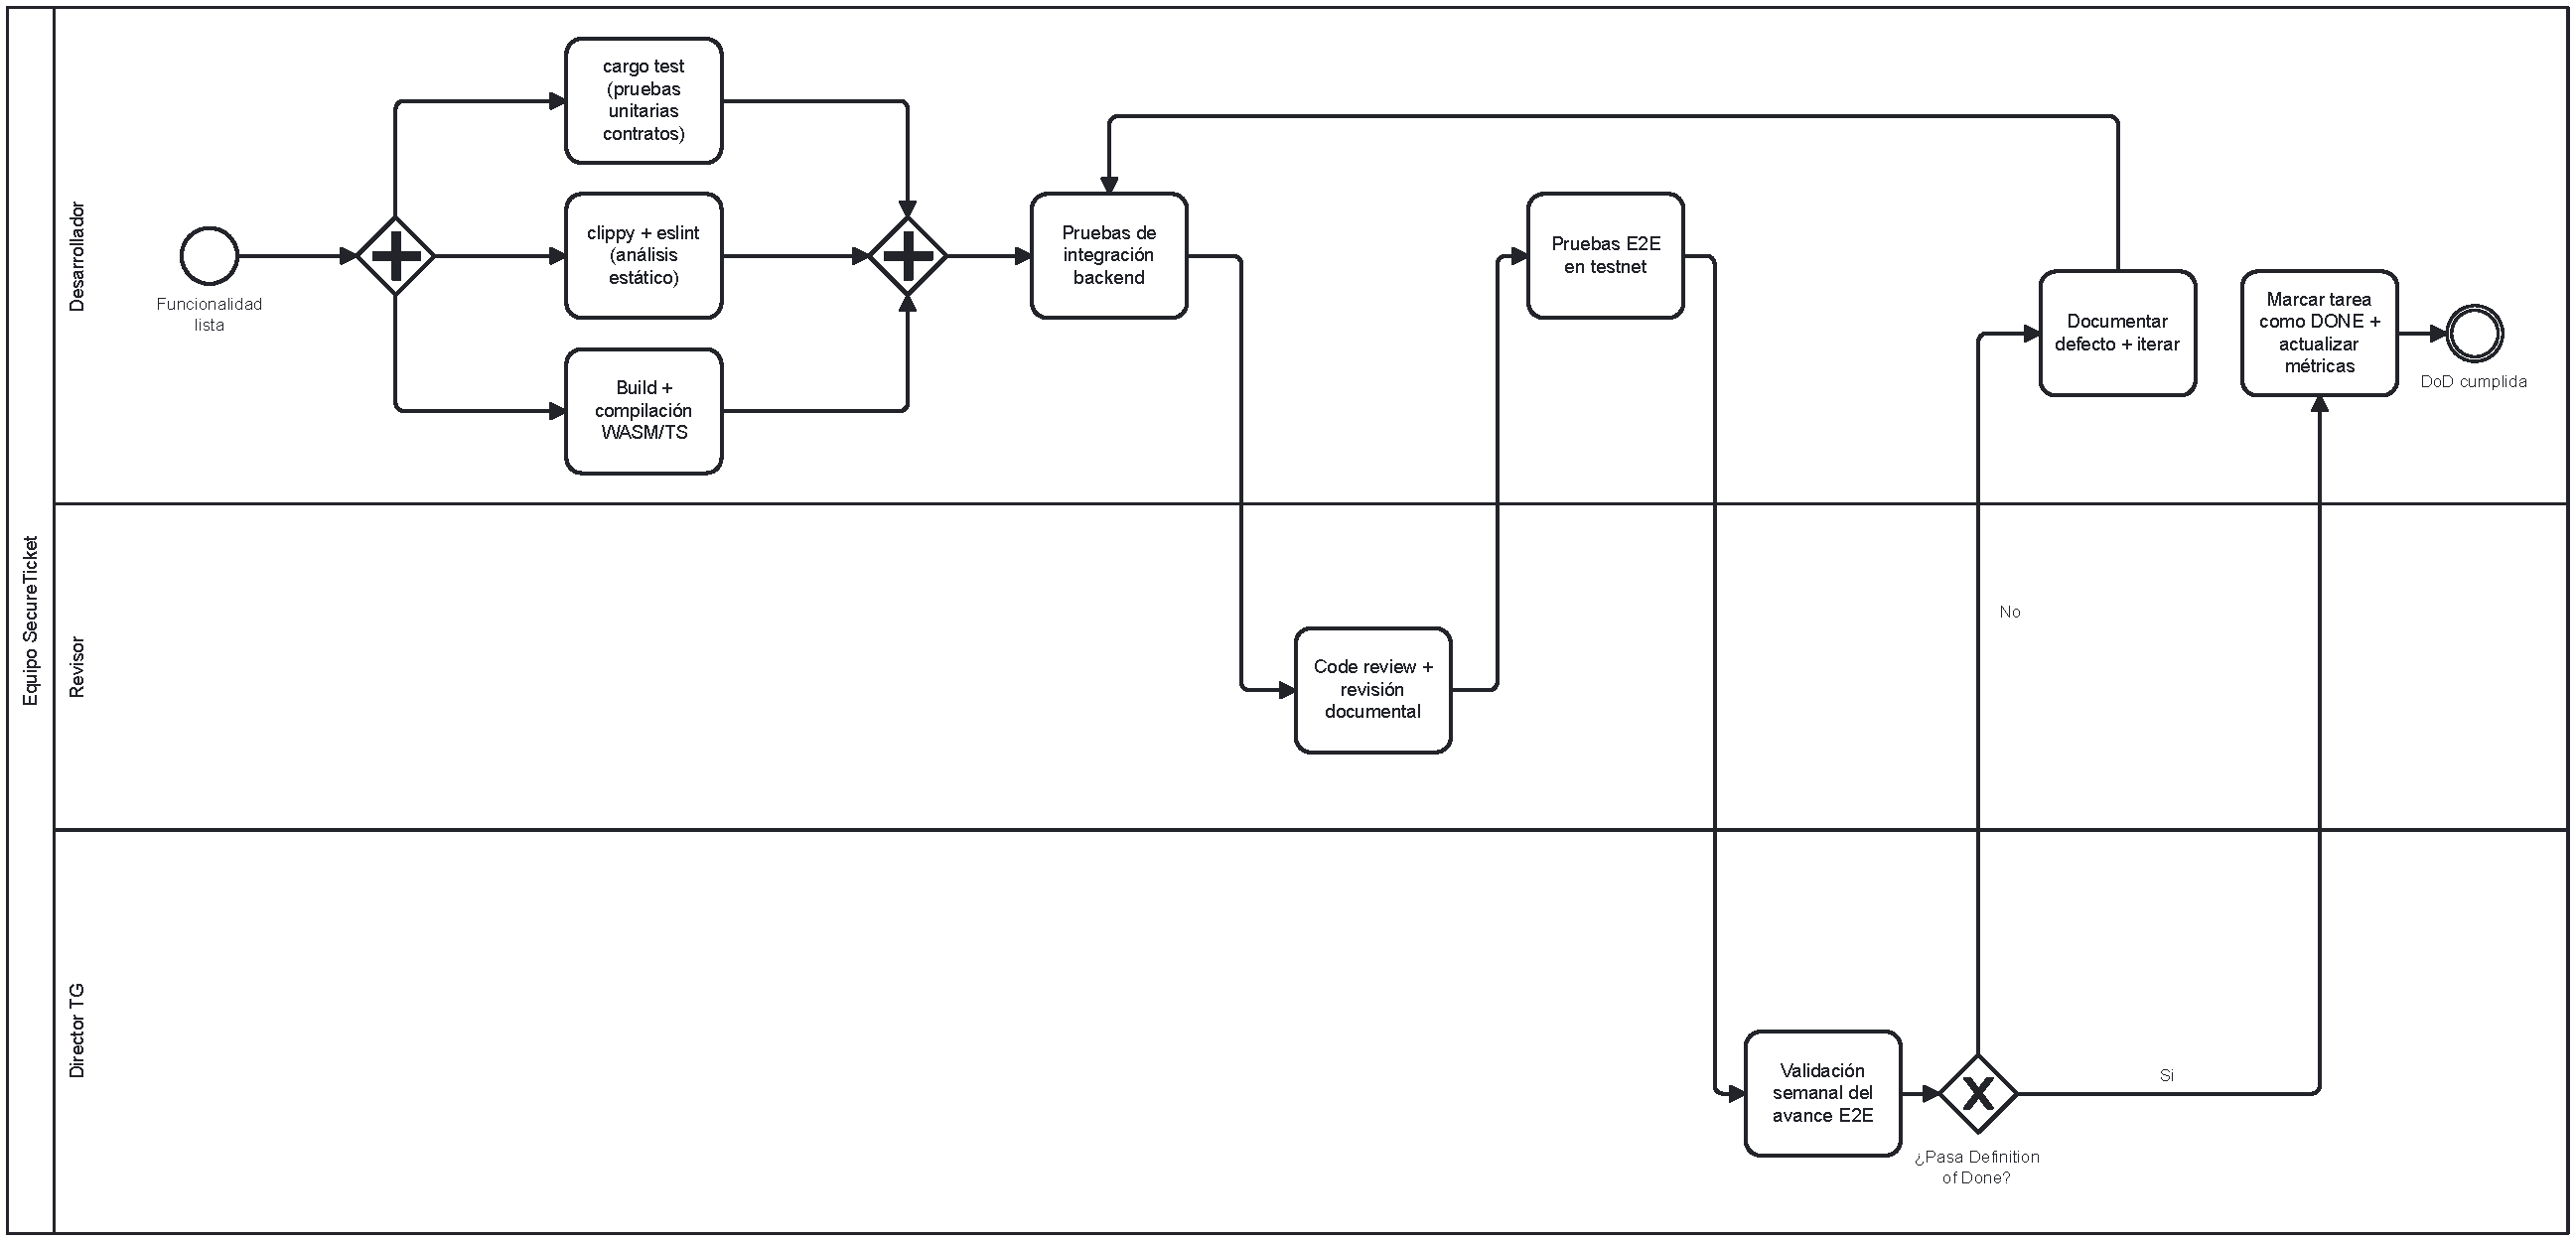
\includegraphics[width=0.95\linewidth]{diagrams/bpmn-calidad.pdf}
        \caption{Flujo BPMN de control de calidad — verificación paralela, validación y revisiones.}
        \label{fig:bpmn-calidad}
      \end{figure}

      \subsubsection{Verificación}
      \begin{itemize}
        \item \textbf{Pruebas unitarias} en cada función pública de los contratos (Rust \texttt{\#[test]}).
        \item \textbf{Pruebas de integración} en el backend, cubriendo rutas críticas (autenticación, \textit{checkout}, operaciones on-chain).
        \item \textbf{Pruebas E2E} desde el frontend cubriendo el flujo: compra Web2 $\rightarrow$ asegurar on-chain $\rightarrow$ reventa P2P $\rightarrow$ verificación en puerta.
        \item \textbf{Análisis estático:} \texttt{cargo clippy} y \texttt{cargo fmt} en Rust; \texttt{tsc --noEmit} y \texttt{eslint} en TypeScript.
        \item \textbf{Verificación de \textit{builds}:} compilación local exitosa antes de cada \textit{pull request}.
      \end{itemize}

      \subsubsection{Validación}
      \begin{itemize}
        \item \textbf{Validación con el director:} demostración semanal del avance E2E sobre la \textit{testnet}.
        \item \textbf{Validación contra criterios de aceptación del SRS:} antes del cierre de cada fase incremental.
        \item \textbf{Validación cruzada del equipo:} cada integrante valida los flujos cuya implementación no le pertenece, para reducir sesgos del autor.
        \item \textbf{Validación final:} ejecución del flujo E2E completo en \textit{testnet} con los 12 eventos desplegados.
      \end{itemize}

      \subsubsection{Revisiones e inspecciones}
      \begin{itemize}
        \item \textbf{Revisión por pares (\textit{code review})} en todo \textit{pull request}: al menos un revisor distinto al autor.
        \item \textbf{Revisión de documentos:} revisiones cruzadas entre integrantes antes de marcar un documento como final.
        \item \textbf{Revisión con el director:} validación semanal del estado de los artefactos académicos y del prototipo.
        \item \textbf{Inspección de configuración:} verificación periódica de que no haya secretos en el repositorio público.
      \end{itemize}

      \subsubsection{Definition of Done (DoD)}
      Una tarea o entregable se considera \textbf{hecho} cuando cumple, según aplique:
      \begin{itemize}
        \item Código en \texttt{main} mediante \textit{pull request} aprobado.
        \item Pruebas asociadas al cambio pasando al $100\%$.
        \item Documentación actualizada (si la funcionalidad lo amerita).
        \item No introduce regresiones en los flujos E2E ya estables.
        \item Para documentos académicos: revisión cruzada interna y, si aplica, validación con el director.
      \end{itemize}

      \subsubsection{Resumen de resultados de calidad}
      Al cierre del proyecto, los principales indicadores de calidad son:
      \begin{itemize}
        \item \textbf{58/58 pruebas} de contratos aprobadas (Sección~\ref{subsec:monitoreo-progreso}).
        \item \textbf{100\%} de funciones públicas de los contratos cubiertas por al menos una prueba.
        \item \textbf{12/12 eventos} desplegados y verificables en \textit{testnet}.
        \item \textbf{0 defectos críticos} abiertos.
        \item \textbf{Seis documentos académicos} revisados internamente y validados con el director.
      \end{itemize}

  % =========================================================
  %  Anexos
  % =========================================================
  \section*{Anexos}
  \addcontentsline{toc}{section}{Anexos}
  \label{sec:anexos}
    Este documento es \textbf{autocontenido}: toda la información operativa, métricas, cronograma, riesgos y procesos necesarios para entender la gestión del proyecto se encuentra dentro de las secciones~6 a~12. Los siguientes elementos complementarios se mantienen como artefactos vivos en el repositorio del trabajo de grado:
    \begin{itemize}
      \item \textbf{Tablero Kanban} (GitHub Projects): historial de tarjetas, \textit{lead time} y \textit{cycle time} por tarjeta. Repositorio: \url{https://github.com/Tesis-Stellar}.
      \item \textbf{Hoja de horas-persona} (Google Drive): registro semanal por integrante, base de la métrica de desviación de esfuerzo (Sección~\ref{subsec:monitoreo-progreso}).
      \item \textbf{Bitácora de revisiones semanales con el director}: actas breves de cada reunión (15--16 actas).
      \item \textbf{Salida de pruebas} (\texttt{cargo test}, \texttt{npm test}): logs completos de las 58 pruebas de contratos y las pruebas E2E del backend/frontend.
      \item \textbf{Reportes de despliegue en \textit{testnet}}: hashes de transacción y direcciones de los 12 contratos de evento desplegados.
    \end{itemize}
    Estos artefactos no se incluyen en línea para mantener la legibilidad del documento, y son consultables bajo solicitud al equipo o al director del trabajo de grado.

  % =========================================================
  %  Referencias
  % =========================================================
  \section*{Referencias}
  \addcontentsline{toc}{section}{Referencias}
  \label{sec:referencias}
    \begin{thebibliography}{99}
      \bibitem{ieee1058} IEEE Std 1058-1998, \textit{IEEE Standard for Software Project Management Plans}, 1998.
      \bibitem{iso16326} ISO/IEC/IEEE 16326:2009, \textit{Systems and software engineering — Life cycle processes — Project management}, 2009.
      \bibitem{iso12207} ISO/IEC/IEEE 12207:2017, \textit{Systems and software engineering — Software life cycle processes}, 2017.
      \bibitem{pmbok2021} Project Management Institute, \textit{A Guide to the Project Management Body of Knowledge (PMBOK Guide)}, 7th ed., 2021.
      \bibitem{puj2025} Pontificia Universidad Javeriana, \textit{Guía y plantilla del curso para SPMP}, 2025.
      \bibitem{royce1970} W. W. Royce, ``Managing the development of large software systems,'' in \textit{Proc. IEEE WESCON}, 1970, pp. 1--9.
      \bibitem{kruchten2003} P. Kruchten, \textit{The Rational Unified Process: An Introduction}, 3rd ed., Addison-Wesley, 2003.
      \bibitem{schwaber2020} K. Schwaber and J. Sutherland, \textit{The Scrum Guide}, 2020. \url{https://scrumguides.org/}.
      \bibitem{anderson2010} D. J. Anderson, \textit{Kanban: Successful Evolutionary Change for Your Technology Business}, Blue Hole Press, 2010.
      \bibitem{brechner2015} E. Brechner, \textit{Agile Project Management with Kanban}, Microsoft Press, 2015.
      \bibitem{beck2002} K. Beck, \textit{Test-Driven Development: By Example}, Addison-Wesley, 2002.
      \bibitem{humble2010} J. Humble and D. Farley, \textit{Continuous Delivery}, Addison-Wesley, 2010.
      \bibitem{stellardocs} Stellar Development Foundation, \textit{Stellar Documentation}, \url{https://developers.stellar.org/}.
      \bibitem{sorobandocs} Stellar Development Foundation, \textit{Soroban Smart Contracts Documentation}, \url{https://soroban.stellar.org/}.
      \bibitem{wood2014} G. Wood, ``Ethereum: A secure decentralised generalised transaction ledger,'' \textit{Ethereum Yellow Paper}, 2014.
      \bibitem{solidity} Ethereum Foundation, \textit{Solidity Documentation}, \url{https://docs.soliditylang.org/}.
      \bibitem{solanadocs} Solana Foundation, \textit{Solana Documentation}, \url{https://docs.solana.com/}.
      \bibitem{movebook} S. Blackshear et al., \textit{Move: A Language With Programmable Resources}, Diem, 2019.
      \bibitem{klabnik2023} S. Klabnik and C. Nichols, \textit{The Rust Programming Language}, 2nd ed., No Starch Press, 2023.
      \bibitem{reactdocs} Meta, \textit{React Documentation}, \url{https://react.dev/}.
      \bibitem{vitedocs} E. You, \textit{Vite Documentation}, \url{https://vitejs.dev/}.
      \bibitem{vuedocs} E. You, \textit{Vue.js Documentation}, \url{https://vuejs.org/}.
      \bibitem{sveltedocs} R. Harris, \textit{Svelte Documentation}, \url{https://svelte.dev/}.
      \bibitem{expressdocs} OpenJS Foundation, \textit{Express Documentation}, \url{https://expressjs.com/}.
      \bibitem{prismadocs} Prisma, \textit{Prisma ORM Documentation}, \url{https://www.prisma.io/docs}.
      \bibitem{springdocs} VMware, \textit{Spring Boot Documentation}, \url{https://spring.io/projects/spring-boot}.
      \bibitem{djangodocs} Django Software Foundation, \textit{Django Documentation}, \url{https://docs.djangoproject.com/}.
      \bibitem{postgresdocs} PostgreSQL Global Development Group, \textit{PostgreSQL Documentation}, \url{https://www.postgresql.org/docs/}.
      \bibitem{supabasedocs} Supabase, \textit{Supabase Documentation}, \url{https://supabase.com/docs}.
      \bibitem{mongodocs} MongoDB, \textit{MongoDB Documentation}, \url{https://www.mongodb.com/docs/}.
      \bibitem{freighter} Stellar Development Foundation, \textit{Freighter Wallet}, \url{https://www.freighter.app/}.
      \bibitem{awsdocs} Amazon Web Services, \textit{AWS Documentation}, \url{https://docs.aws.amazon.com/}.
      \bibitem{verceldocs} Vercel, \textit{Vercel Documentation}, \url{https://vercel.com/docs}.
      \bibitem{railwaydocs} Railway, \textit{Railway Documentation}, \url{https://docs.railway.app/}.
    \end{thebibliography}

\end{document}